\chapter{Implementierung und konkrete Algorithmusbestandteile}\label{ch:impl}

Dieses Kapitel steigt in das Detail: zuerst die Repository-Architektur mit der Träger-Stufenkette
(Abschnitt~\ref{sec:anatomy-levels}) und den vier Arbeitsmodi einer Permutation, dann jede Schlüsselstelle
von PRT-ART einzeln und bildhaft, anschließend die Achsen-Implementierung mit der \emph{einen} Architektur
im Code, der Code-Gestalt der Bau-Kette, den Ebenen E4--E0 im Code und den Vertrags-Flächen an den
Träger-Binaries, danach die Qualitätssicherung über Contract-Tests je Schicht samt Zwei-Gate-Protokoll
und die Code-Gestalt der Realm-Wurzeln --- System- und Mess-Achsen einschließlich der Hardware-Erkennung ---
und zuletzt das Register der Entwurfsmuster, die Hybrid-Stufe und das Lager. Im Kern ist die \emph{eine}
Architektur eine selbst-optimierende Compiler-Compiler-Struktur: Der Planer erzeugt aus der Anwender-XML
die Bau-Aufträge, der Builder erzeugt daraus die Kompilate, und die Auswertung der Messwerte speist die
nächste Planung (Abschnitt~\ref{sec:mess-chain}). Damit steht der Apparat in der Linie der empirischen
Autotuning-Systeme, die Kandidaten-Implementierungen erzeugen, vermessen und die Auswahl aus den Messwerten
treffen~\cite{whaley2001atlas,frigo1998fftw,ansel2014opentuner,balaprakash2018autotuning}; der Unterschied
liegt darin, dass hier nicht die Parameter einer festen Implementierung, sondern die Organ-Belegung eines
Lebewesens permutiert und je Permutation eine eigene Binary erzeugt wird.

%% INTERN-272: KA-055
\section{Vier-Repository-Architektur}\label{sec:repos}
Die Implementierung verteilt sich auf vier Git-Repositorien mit klar getrennten Verantwortlichkeiten:
\begin{itemize}
  \item \texttt{comdare-cache-engine} --- \textbf{wie} gemessen wird: die Bausteine-Bibliothek und der
  Builder (XML-Config-Parser, \texttt{generate\_\allowbreak{}module\_\allowbreak{}from\_\allowbreak{}profile}-Codegenerierung,
  Permutations-Schleife, Modul-Loader, der siebenphasige \texttt{ExperimentDriver} mit den Phasen
  \texttt{phase1\_enumerate} bis \texttt{phase7\_export} und der Experiment-Planer
  \texttt{ExperimentPlanDirector}, Abschnitt~\ref{sec:impl-pipeline}); die ABI-Header unter \texttt{abi/}
  --- der lebende ABI-Kern \texttt{module\_\allowbreak{}abi\_\allowbreak{}v1} sowie der vom Bau isolierte
  Test-Cluster aus \texttt{baustein\_\allowbreak{}variants} und \texttt{resolve\_\allowbreak{}baustein}
  (Abschnitt~\ref{sec:axes-impl}) ---; die 33~SOTA-Profile unter
  \texttt{algorithm\_\allowbreak{}profiles/\allowbreak{}sota} als ausführbare XML --- 30~Vollprofile und
  drei abstrakte Profile (Abschnitt~\ref{sec:sota-instances}) --- und die Test-Suites. Die Bibliothek \texttt{search\_\allowbreak{}engine} ist ein deklariertes, inhaltsleeres
  Skelett (siebzehn Dateien, davon acht Platzhalter und neun Bau-Beschreibungen ohne Quellcode), und
  \texttt{execution\_\allowbreak{}engine} enthält drei Inhaltsdateien (Ergebnis-Aggregator und
  Experiment-Demonstration); die lebende Wurzel der Ausführungs-Engine liegt unter
  \texttt{libs/\allowbreak{}cache\_\allowbreak{}engine/\allowbreak{}execution\_\allowbreak{}engine}
  (Abschnitt~\ref{sec:impl-architecture}). Der Quellbaum folgt einem Pitchfork-Layout (\texttt{apps/} für
  ausführbare Dateien, \texttt{libs/} für Bibliotheken, \texttt{libs/common} für querschnittlichen Code);
  hinzu treten \texttt{libs/traeger} mit den vier Träger-Stufen (unten),
  \texttt{libs/\allowbreak{}cache\_\allowbreak{}engine/\allowbreak{}heuristik} mit sechs Headern (Achsen-Spline,
  Break-Even, Messkurven-Lader, Offline-Clusterung der Workloads, Merkmalsvektor, Optimierungs-Katalog) und
  \texttt{libs/test\_infra} (Benchmark-Suite, Workload-Generator, Testdaten).
  \item \texttt{comdare-prt-art} --- der \textbf{Prüfling}: die hybride \texttt{PrtArtSearchEngine} mit
  der 1/2/N-Parameter-Regel (ein Parameter fordert die Funktionsinterfaces eines Vektors, zwei die einer
  Map, mehr als zwei die einer Map auf ein Tupel), ihre ABI-Adapter und ihre Bausteine
  (4+1+2-Allokator-Pools --- sieben Pools: vier Seiten-Pools mit den Rollen Trie-Hülle, Dense-Pages,
  MultiLevel und Decision-Span, ein Rest-Pool und zwei Wert-Pools für statische und dynamische Werte ---,
  OLC mit reservierten Blöcken, MultiLevel-Layout, pfadorientiertes Prefetch, DensityTracker,
  Hypothesen-Metriken H1/H2/H3) sowie die prüflingseitigen Vergleichs-Re-Implementierungen der
  Rang-2/3-Arbeiten (\texttt{legacy\_\allowbreak{}reimpl}, vierzehn Verzeichnisse P11--P27 ohne P15, P20
  und P25), die im SOTA-Beitrittstest gegen die tatsächlichen Adapter der Cache-Engine verglichen werden ---
  Rang~1 (Zentralitäts-Rang, Abschnitt~\ref{sec:rqs}) umfasst die acht eigenständigen Suchentwürfe
  --- alle mit öffentlichem Quellcode und Original-Adapter --- sowie die als Organe eingehenden
  Arbeiten P08 und P09; von den Rang-2/3-Arbeiten besitzen P20, P25, P29 und P30 ebenfalls
  Original-Adapter über \texttt{ext/}, die vierzehn Arbeiten in \texttt{legacy\_\allowbreak{}reimpl}
  sind ohne öffentlichen Quellcode nach der Veröffentlichung re-implementiert
  (Abschnitt~\ref{sec:sota-instances}). Pool-, Prefetch- und Layout-Komponenten sind Deskriptor-Skelette
  ohne eigene Speicheranbindung; welche Prüflings-Bausteine den Mess-Apparat erreichen, entscheidet die
  Slot-Belegung (Abschnitt~\ref{sec:prtart-impl}).
  \item \texttt{probst-Diplomarbeit-cache-engine} --- \textbf{was} durch den Anwender getestet wird: die
  Experiment-Konfigurationen (XML samt XSD-Schema), der Mess-Treiber \texttt{messung\_driver} (Binary
  \texttt{comdare-messung-driver}, die CEB-Rolle) und die Auswertungs-Werkzeugkette aus neun numerierten
  Programmen von \texttt{01\_\allowbreak{}sample\_\allowbreak{}data\_\allowbreak{}generator} bis
  \texttt{09\_\allowbreak{}tex\_\allowbreak{}formatter}
  (Abbildung~\ref{fig:toolchain}).
  \item das \textbf{Manuskript-Repository} --- die versionierte Experimentdurchführung direkt im Dokument:
  Die Generator-Ausgabe der Werkzeugkette (Tabellen- und Diagramm-Dateien je Messreihe) wird per Commit
  unter \texttt{anhang/<sprache>/tabellen/} abgelegt und vom Manuskript eingebunden, das Repository besitzt
  eine eigene CI mit den Jobs \texttt{lint:secrets}, \texttt{lint:latex} und \texttt{thesis:pdf}, und das
  Projekt-Repository stößt den Manuskript-Bau nach einem Messlauf an (\texttt{trigger:thesis}). Ein
  Messwert im Dokument ist damit ein versionierter Artefakt-Stand mit Herkunft, kein abgeschriebener Wert
  --- das ist der Grund, warum das Manuskript ein eigenes Git-Repository mit eigener Pipeline ist.
\end{itemize}
Die Vierer-Ordnung des Codes ist nicht die Repository-Grenze, sondern die \emph{Träger-Stufenkette}
Planer $\to$ CEB $\to$ Tier $\to$ Hybrid (Abschnitt~\ref{sec:anatomy-levels}): Der Stempel-Vertrag kennt
genau vier Träger in dieser Reihenfolge, und der Quellbaum bildet sie unter \texttt{libs/traeger} als vier
Unterprojekte in Stufenform ab --- \texttt{comdare\_planner}, \texttt{comdare\_ceb},
\texttt{comdare\_tier\_emission} und \texttt{comdare\_hybrid} ---, wobei Stufe $N+1$ nur an Stufe $N$ hängt,
nie umgekehrt, und jede Stufe mit einer strikten Konfigurationsprüfung auf ihre Vorstufe schließt.
Umsetzungsstand dieser Ordnung: Die Unterprojekte bilden ein Gerüst (je Stufe Bau-Beschreibung und
Beschreibungsdatei, Planer und CEB mit eigenem Include-Verzeichnis), und die eigentliche Implementierung liegt
als Monolith unter \texttt{libs/\allowbreak{}cache\_\allowbreak{}engine}; ihre Aufteilung entlang der Stufen
ist vorgesehen, aber nicht umgesetzt. Der Prüfling ist keine Stufe, sondern der quer liegende Lieferant von
Organ-Bausteinen; Builder und CacheEngine teilen sich das Engine-Repository --- der Builder als ausführbare
Datei (\texttt{apps/}) über seiner Builder-Bibliothek
(\texttt{libs/\allowbreak{}cache\_\allowbreak{}engine/\allowbreak{}builder}), die CacheEngine als Bibliothek
(\texttt{libs/\allowbreak{}cache\_\allowbreak{}engine}). Die Stufenkette ist zugleich die Schicht, an deren
Binaries die Verträge in Flächen zergliedert sind (Abschnitt~\ref{sec:impl-pipeline});
Abbildung~\ref{fig:traeger-stufen} zeigt sie mit ihren Binaries, Legenden-Formen und Flächen.
\begin{figure}[htbp]\centering
%% INTERN-272: KA-056
\begin{tikzpicture}[font=\footnotesize,>=Stealth,
  st/.style={draw,rounded corners,fill=blue!7,minimum width=3.75cm,minimum height=3.9cm,text width=3.55cm,align=center,inner sep=3pt},
  fl/.style={draw,rounded corners,fill=orange!10,minimum width=3.75cm,minimum height=1.35cm,text width=3.55cm,align=center,inner sep=2pt,font=\tiny}]
  \node[st] (s1) at (0,0){\textbf{Stufe 1: Planer}\\{\tiny\texttt{comdare-experiment-planner}}\\[2pt]{\tiny löst die Anwender-XML gegen die drei Kataloge auf; Director-Walk; Legende \texttt{ceb:build:\allowbreak[a,b,c]}}};
  \node[st] (s2) at (3.95,0){\textbf{Stufe 2: CEB}\\{\tiny\texttt{comdare-messung-driver}}\\[2pt]{\tiny führt die Mess-Wahl einkompiliert, permutiert System $\times$ Organ; Legende je Host \texttt{tier:build-batch:\allowbreak<host>}, Testate \texttt{zelle=\allowbreak[d,e,f]\allowbreak[g,h,i]}}};
  \node[st] (s3) at (7.9,0){\textbf{Stufe 3: Tier}\\{\tiny\texttt{comdare\_perm\_<fp>.so}}\\[2pt]{\tiny eine Organ-Permutation je Binary; sieben Pflicht-Symbole; Mess-Batch je Host \texttt{measure:\allowbreak[a,b,c]:\allowbreak batch:\allowbreak<host>}, Mess-Testate \texttt{zelle=\allowbreak[a,b,c]\allowbreak[d,e,f]\allowbreak[g,h,i]}}};
  \node[st] (s4) at (11.85,0){\textbf{Stufe 4: Hybrid}\\{\tiny Hybrid-\texttt{.so}}\\[2pt]{\tiny dieselben Pflicht-Symbole; Dock-Array mit angeschlossenen Tieren; \texttt{genus()} meldet den Ziel-Genus}};
  \draw[->,thick] (s1)--(s2); \draw[->,thick] (s2)--(s3); \draw[->,thick] (s3)--(s4);
  \node[fl] (f1) at (0,-2.95){Fläche 2 (Stempel): Selbst-Version X.Y.Z, Fingerprint SHA-256, Gesamt-Stempel};
  \node[fl] (f2) at (3.95,-2.95){Fläche 2 (Stempel): Mess- und System-Zeile, Fingerprint SHA-512; eigene Mess-Gate-Belegung};
  \node[fl] (f3) at (7.9,-2.95){Flächen 1--3: Genus-Interface, Stempel (drei Zeilen), Mess-Durchstich \texttt{IMessVisitor}};
  \node[fl] (f4) at (11.85,-2.95){Flächen 1--3 wie Tier, dazu die angeschlossenen Stempel-Zeilen (Laufzeit-Haken)};
  \draw[dashed,gray] (s1)--(f1); \draw[dashed,gray] (s2)--(f2); \draw[dashed,gray] (s3)--(f3); \draw[dashed,gray] (s4)--(f4);
\end{tikzpicture}
\caption[Die Träger-Stufenkette im Code]{Die Träger-Stufenkette im Code: vier Träger in fester Reihenfolge (Stempel-Vertrag), je Stufe die
Binary, ihre Legenden-Form in der emittierten Pipeline und die an ihr ausgeprägten Vertrags-Flächen.
Stufe $N+1$ hängt nur an Stufe $N$; nur die Mess-Testate enthalten alle drei Achsen-Klammern. Die Flächen
zergliedern die Verträge (Abschnitt~\ref{sec:impl-pipeline}); die Unterprojekte unter \texttt{libs/traeger}
sind ein Gerüst, die Implementierung liegt als Monolith unter \texttt{libs/cache\_engine}.}\label{fig:traeger-stufen}
\end{figure}
Quer dazu trennt die Terminologie zwei Engine-Begriffe, die nicht kurzgeschlossen werden dürfen. Die
\texttt{CacheEngine} (\texttt{libs/\allowbreak{}cache\_\allowbreak{}engine}) ist die \emph{Bibliothek der Achsen-Bausteine}:
Sie stellt je Achse die austauschbaren Entwurfsbestandteile als Concept-/CRTP-Komponenten
bereit\footnote{CRTP\@: das \emph{Curiously Recurring Template Pattern}~\cite{coplien1995crtp}, der statische
Polymorphismus, bei dem eine Klasse von einer Klassenschablone abgeleitet wird, der sie sich selbst als
Schablonenargument übergibt (Abschnitt~\ref{sec:software-means}); virtuelle Aufrufe werden so durch statisch
aufgelöste ersetzt.} und enthält \emph{keine} Mess-Logik. Die \texttt{ExecutionEngine} hingegen ist die quer
zu allen Achsen liegende \emph{Ausführungs- und Mess-Infrastruktur}: Ihre abstrakte messbare Wurzel ist
\texttt{IExecutionEngine} (Abschnitt~\ref{sec:measurement-system}) mit den drei Engine-Arten Anatomy, Virus
und Hybrid; der konkrete Laufzeit-Adapter \texttt{SearchAlgorithmAbiAdapter<A>} liefert über die
\texttt{SearchAlgorithmAnatomy} die OS-Primitiven (cache-line-ausgerichtete Allokation, NUMA-konformes
Read-Pinning, kohärenz-bewusstes Schreiben); die Mess- und Observer-Kopplungen des Adapters werden über
\texttt{COMDARE\_\allowbreak{}MEASUREMENT\_\allowbreak{}ON} geschaltet, und den Mess-Aggregator führt der
\texttt{ExperimentDriver} host-seitig; die CMake-Option
\texttt{COMDARE\_\allowbreak{}EXPERIMENT\_\allowbreak{}MODE} markiert Experiment-Kompilate und kodiert
übersetzungszeitlich die Invariante, dass ein Experiment-Bau stets ein Mess-Bau ist --- sie selbst
schaltet keine Hooks, und ein Experiment-Bau ohne Mess-Modus bricht die Konfiguration. Kurz: Die
\texttt{CacheEngine} liefert die \emph{Bausteine}, die \texttt{ExecutionEngine} die \emph{Werkzeuge}; diese
Trennung hält den Produktiv-Pfad mess-frei.

Was mit einer Permutation geschieht, ist eine Registry und kein Etikett: Die vier \emph{Arbeitsmodi}
(work modes) \texttt{build}, \texttt{measure}, \texttt{compare} und \texttt{release} sind als Unter-Achse des
Mess-Realms geführt (Tabelle~\ref{tab:work-modes}; Enum-Index, Ablauf-Ordnung und Registry-Zeile sind
dieselbe Reihenfolge, Abschnitt~\ref{sec:anatomy-levels}). \texttt{build} baut die Binaries, ohne zu messen,
und darf parallel laufen; \texttt{measure} ist der deterministische Ein-Thread-Messlauf und der einzige
Modus mit eingeschalteter Messung; \texttt{compare} liest das Messwertlager und vergleicht bereits
gemessene Sichten --- die Stufe \emph{vor} dem Release; \texttt{release} erzeugt die Referenz-Binary ohne
Instrumentierung. Alle vier bauen als CMake-Release; ein messendes Debug-Regime existiert nicht mehr, weil
parallel erhobene Zahlen mit Ein-Thread-Messungen nicht vergleichbar sind, und der Verdrahtungs-Check, den
es leistete, ist als Schalter \texttt{--debug} der Planer-Shell realisiert --- ein Flag, kein Zustand.
Umsetzungsstand: \texttt{compare} ist ein wählbares Etikett mit \texttt{release}-gleicher Bausemantik;
sein modus-spezifischer Ablauf (Replay-Vergleich statt Messen) ist vorgesehen, aber nicht
implementiert (Abschnitt~\ref{sec:anatomy-levels}).
\begin{table}[htbp]\centering\footnotesize
\begin{tabular}{@{}llllp{5.6cm}@{}}
\toprule
Modus & CMake-Typ & misst & Mess-Threads & Zweck / Stand \\
\midrule
\texttt{build}   & Release & nein & --- & Bau ohne Messung, parallel; der Schritt vor jeder Messung \\
\texttt{measure} & Release & ja   & 1   & deterministischer Messlauf, Run-to-Run-stabil; füllt das Messwertlager \\
\texttt{compare} & Release & nein & --- & liest das Messwertlager, Stufe vor \texttt{release}; Ablauf vorgesehen, nicht implementiert (Etikett) \\
\texttt{release} & Release & nein & --- & Referenz-Binary ohne Mess-Instrumentierung \\
\bottomrule
\end{tabular}
\caption{Die vier Arbeitsmodi einer Permutation als registrierte Unter-Achse des Mess-Realms
(\texttt{WorkMode}, vier Einträge; ein fünfter bricht die Übersetzung). Kein Modus misst parallel; nur
\texttt{measure} schaltet die Messung ein.}\label{tab:work-modes}
\end{table}

\section{PRT-ART im Detail}\label{sec:prtart-impl}
Aufbauend auf dem Stand der Technik beschreibt dieser Abschnitt jede Schlüsselstelle von PRT-ART einzeln und
bildhaft; je Schlüsselstelle wird zuerst das verwandte Verfahren benannt, aus dem sie hervorgeht.
Pool-Allokation mit rollenreinen Pools steht in der Linie der Größenklassen- und Thread-Heap-Allokatoren
Hoard, jemalloc und mimalloc~\cite{berger2000hoard,evans2006jemalloc,leijen2019mimalloc}; optimistisches
Lock-Coupling ist das Synchronisationsverfahren des ART~\cite{leis2016olc}; Software-Prefetch entlang der
Baumpfade folgt der Pfad-Bündel-Heuristik der Prefetching-B\textsuperscript{+}-Bäume von Chen, Gibbons und
Mowry~\cite{chen2001prefetch} (die verwandte Literatur des Bausteins im Code) und dem hierarchischen
Prefetching~\cite{zhang2025hierarchical}; cache-line-bewusste
Knoten-Layouts gehen auf den ART und auf FAST zurück~\cite{leis2013art,kim2010fast}; kohärenz-bewusste
Telemetrie beantwortet das False-Sharing-Problem der Mehrprozessor-Caches~\cite{torrellas1994falsesharing}
in der Forschungslinie von Kuehn~\cite{kuehn2023bplustree}. Der DensityTracker und die Hypothesen-Metriken
H1/H2/H3 sind eigene Beiträge ohne Fremdvorlage.

Der Prüfling steuert sechs eigene Schlüsselstellen bei, zwei davon auf der Telemetrie-Achse, die in der
Dreiteilung zweigeteilt ist --- Sweep-Unter-Achse (sub-axis) des Mess-Toolings im Planer und
Übersetzungszeit-Größe im Builder (Abschnitt~\ref{sec:axis-triad}). Auf der \emph{Allokator-Achse} ersetzt
ein \emph{4+1+2-Pool-Allokator} --- vier Seiten-Pools mit den Rollen Trie-Hülle, Dense-Pages, MultiLevel
und Decision-Span, ein Rest-Pool und zwei Wert-Pools für statische und dynamische Werte --- die
algorithmus-fest verdrahtete Allokation durch eine cache-line-ausgerichtete, fragmentierungsarme Free-List.
Auf der \emph{Nebenläufigkeits-Achse} --- selbst gegliedert in Pattern (8.1) und Locking-Mode (8.2) --- trägt
PRT-ART \emph{optimistisches Lock-Coupling (OLC) mit reservierten Wert-Blöcken} bei
(\texttt{olc\_\allowbreak{}with\_\allowbreak{}reserved\_\allowbreak{}blocks}), koordiniert über einen
Concurrency-Manager, der die Disziplinen OLC, Hardware- und Software-Transaktionsspeicher (HTM, STM),
Lock-Free, Read-Copy-Update (RCU) und Hazard Pointers~\cite{michael2004hazard} führt; die Speicherfreigabe
ist dabei eine Unter-Achse des Allokators (epoch-, RCU-, Hazard-Pointer- und QSBR-Strategien je
Permutation wählbar). Auf der \emph{Prefetch-Achse} liefert ein \emph{pfadorientiertes Bundle-Prefetch}
die heißen Suchpfade --- die häufig durchlaufenen Knotenfolgen --- vorab, auf der \emph{Layout-Achse}
ein \emph{MultiLevel-Layout}. Besonders
cache-kritisch ist die \emph{Telemetrie-Achse}: Per-Node-Zähler verursachen auf Mehr-Kern-Systemen
Cache-Line-Ping-Pong und verfälschen genau jene Messungen, die sie erheben. Der
Kuehn-Forschungslinie~\cite{kuehn2023bplustree} folgend bietet PRT-ART daher cache-kohärenz-bewusste
Strategien --- \emph{Leaf-Only-Zähler} (Hauptvariante), \emph{Sampling} (jeder $N$-te Blattzugriff) und
\emph{Offline-Recompute} (Bottom-up-Aggregation vor dem Reordering) ---, während der klassische
Per-Node-Zähler nur als gekennzeichnetes Anti-Pattern erhalten bleibt. Den DensityTracker
(\texttt{density\_\allowbreak{}tracker}) und die Hypothesen-Metriken H1/H2/H3 ergänzt der Prüfling als
eigene Telemetrie-Organe.
%% INTERN-272: KA-057
Im Engine-Quellbaum liegen die Baustein-Implementierungen dieser drei Telemetrie-Strategien (TM1--TM3) und
die ISA-Unter-Achsen (IS1--IS3) unter den Verzeichnissen der Organ-Achsen, während Telemetrie-Regime und
Ziel-ISA in der Registry der System-Achsen geführt werden und die Permutations-Flag-Struktur eine eigene
ISA- und Telemetrie-Bank besitzt (Abschnitt~\ref{sec:impl-pipeline}); diese doppelte Verortung ist Bestand des
Codes, keine Zuordnungsfrage des Modells.

Diese Schlüsselstellen sind \emph{Bausteine des Prüfling-Repos}; welche davon den Mess-Apparat erreichen,
entscheidet die Slot-Belegung, nicht die Beitragsliste (Abschnitt~\ref{sec:prtart-demo}). Der Prüfling
stellt vier Slot-Hüllen: den Seitentyp der Build-Achse (\texttt{PrtArtBPlusPageType}), das Prefetch
(\texttt{PrtArtRedirectPrefetch}, T7), das ChainRef-Wert-Handle (\texttt{PrtArtChainRefHandle}, T10) und
einen Telemetrie-Wrapper mit dem Per-Node-Zähler als Anti-Pattern-Vergleichsbasis. Seine codegen-fähige
Slot-Komposition \texttt{PrtArtCompositionDemo} übernimmt sechzehn der achtzehn Organe aus der
ART-Referenz-Komposition der Cache-Engine und ersetzt genau zwei --- Prefetch und Wert-Handle ---; die
Engine-seitige Referenz-Komposition \texttt{PrtArtComposition} unterscheidet sich von der ART-Komposition
in genau einer Achse, dem Pfadkompressions-Redirect (T3, das \emph{R} in PRT-ART), und erbt das
optimistische Lock-Coupling von ART\@. Im Mess-Apparat überschrieben sind damit Pfadkompressions-Redirect,
Prefetch und Wert-Handle (zusammen mit der Build-Achse Seitentyp); der 4+1+2-Pool-Allokator (T6) und das
MultiLevel-Layout (T5) laufen im Mess-Pfad über den Cache-Engine-Standard, die reservierten
OLC-Wert-Blöcke über die von ART geerbte OLC-Disziplin, und die Telemetrie-Strategien treten als
Mess-Tooling-Unter-Achse auf, nicht als Kompositions-Slot. Die Anbindung von Pool-Allokator und Layout an
den Mess-Pfad ist vorgesehen, aber nicht implementiert (Aktualisierung der Prüfling-Einbindung).
Auf eine Galerie verdichtet zeigt Abbildung~\ref{fig:prtart-gallery} die sechs eigenen Schlüsselstellen
von PRT-ART, je an ihrer Achse verortet. Die verbleibenden zwei der acht Bausteinschichten aus der
Beitragsliste (Abschnitt~\ref{sec:contributions}) --- die Inline-/External-/ChainRef-Wert-Handles und
die Signaling-Bit-Serialisierung --- treten nicht als eigene Galerie-Punkte auf: Erstere stellen den im
Apparat überschriebenen Wert-Handle-Slot (T10), Letztere ist als
\texttt{Var\allowbreak{}Len\allowbreak{}Serialization}-Baustein der Serialisierungs-Achse (T9) mit
Signalisierungsbits in Anhang~\ref{app:blocks} katalogisiert.
\begin{figure}[htbp]\centering
%% INTERN-272: KA-058
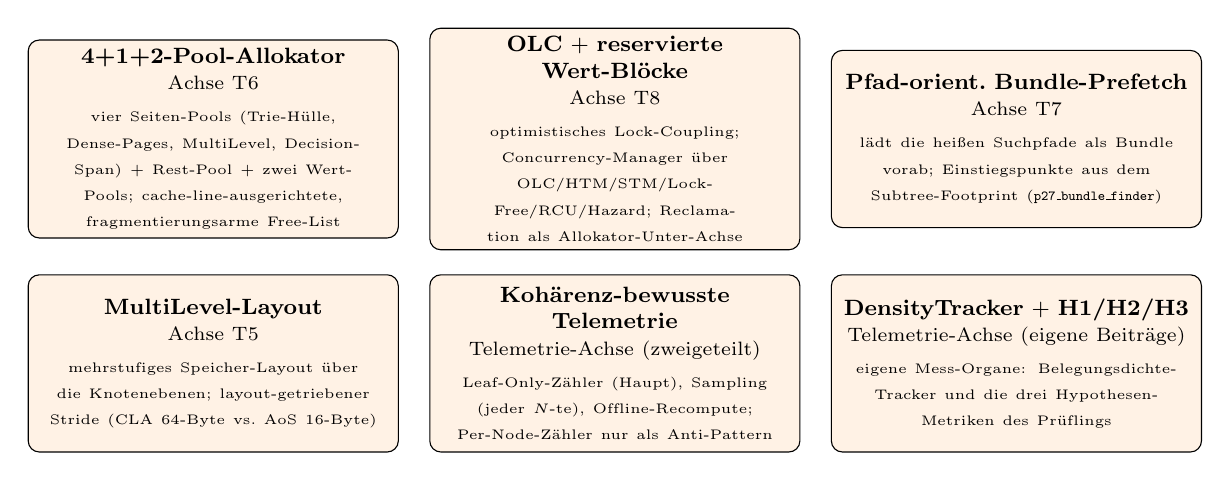
\begin{tikzpicture}[font=\footnotesize,
  pa/.style={draw,rounded corners,fill=orange!10,minimum width=4.7cm,minimum height=2.25cm,text width=4.4cm,align=center,inner sep=3pt}]
  \node[pa] (p1) at (0,0){\textbf{4+1+2-Pool-Allokator}\\{\scriptsize Achse T6}\\[2pt]{\tiny vier Seiten-Pools (Trie-Hülle, Dense-Pages, MultiLevel, Decision-Span) $+$ Rest-Pool $+$ zwei Wert-Pools; cache-line-ausgerichtete, fragmentierungsarme Free-List}};
  \node[pa] (p2) at (5.1,0){\textbf{OLC $+$ reservierte Wert-Blöcke}\\{\scriptsize Achse T8}\\[2pt]{\tiny optimistisches Lock-Coupling; Concurrency-Manager über OLC/HTM/STM/Lock-Free/RCU/Hazard; Reclamation als Allokator-Unter-Achse}};
  \node[pa] (p3) at (10.2,0){\textbf{Pfad-orient.\ Bundle-Prefetch}\\{\scriptsize Achse T7}\\[2pt]{\tiny lädt die heißen Suchpfade als Bundle vorab; Einstiegspunkte aus dem Subtree-Footprint (\texttt{p27\_bundle\_finder})}};
  \node[pa] (p4) at (0,-2.85){\textbf{MultiLevel-Layout}\\{\scriptsize Achse T5}\\[2pt]{\tiny mehrstufiges Speicher-Layout über die Knotenebenen; layout-getriebener Stride (CLA 64-Byte vs.\ AoS 16-Byte)}};
  \node[pa] (p5) at (5.1,-2.85){\textbf{Kohärenz-bewusste Telemetrie}\\{\scriptsize Telemetrie-Achse (zweigeteilt)}\\[2pt]{\tiny Leaf-Only-Zähler (Haupt), Sampling (jeder $N$-te), Offline-Recompute; Per-Node-Zähler nur als Anti-Pattern}};
  \node[pa] (p6) at (10.2,-2.85){\textbf{DensityTracker $+$ H1/H2/H3}\\{\scriptsize Telemetrie-Achse (eigene Beiträge)}\\[2pt]{\tiny eigene Mess-Organe: Belegungsdichte-Tracker und die drei Hypothesen-Metriken des Prüflings}};
\end{tikzpicture}
\caption{Galerie der sechs eigenen Schlüsselstellen von PRT-ART, je an ihrer Achse: ein 4+1+2-Pool-Allokator (T6), optimistisches Lock-Coupling mit reservierten Wert-Blöcken (T8), pfad-orientiertes Bundle-Prefetch (T7), ein MultiLevel-Layout (T5) und cache-kohärenz-bewusste Telemetrie samt DensityTracker und den Hypothesen-Metriken H1/H2/H3 --- die Telemetrie-Achse ist zweigeteilt, Sweep-Unter-Achse des Mess-Toolings und Übersetzungszeit-Größe des Builders (Abschnitt~\ref{sec:axis-triad}). Die Kacheln zeigen die \emph{Bausteine des Prüfling-Repos}; im Apparat überschrieben sind der Pfadkompressions-Redirect (T3, Engine-seitige Referenz-Komposition), das Prefetch (T7) und das ChainRef-Wert-Handle (T10, Slot-Komposition des Prüflings) sowie die Build-Achse Seitentyp; die Bausteine zu T5/T6 laufen im Mess-Pfad über den Cache-Engine-Standard, OLC ist von ART geerbt, und die übrigen Organ-Achsen bezieht die Slot-Komposition aus der ART-Referenz der Cache-Engine (sechzehn von achtzehn).}\label{fig:prtart-gallery}
\end{figure}

\section{Achsen-Implementierung und Mess-System-Ebenen}\label{sec:axes-impl}
Jede Achse wird als generalisiertes Interface implementiert; daneben liegen die Ebenen des Mess-Systems von der
Codegenerierung bis zur Sieben-Phasen-Pipeline. Der Abschnitt schließt mit dem Ebenen-Bild E4--E0 im Code
(Abbildung~\ref{fig:impl-layers}) und den Vertrags-Flächen an den Träger-Binaries; das Register der
verwendeten Entwurfsmuster folgt am Kapitelende (Abbildung~\ref{fig:muster}).
Jede Achse ist ein Topic-Verzeichnis, das ein zweischichtiges \emph{Concept}~\cite{sutton2012concepts} (ein
breites Topic-Concept und ein enges Achsen-Concept) sowie eine durch eine \texttt{requires}-Klausel
abgesicherte \emph{CRTP-Basisklasse} enthält. Der Live-Weg der Baustein-Auswahl ist monomorph: Je Achse
führt eine vollständige Typliste aller bekannten Bausteine (\texttt{All*}), aus der ein
Übersetzungszeit-Filter über das Enable-Flag jedes Bausteins (\texttt{mp\_filter<is\_enabled>},
Boost.Mp11~\cite{dimov_mp11}) die \texttt{Enabled*}-Liste bildet, und eine Composition belegt je Slot genau
einen Typ dieser Liste. Der Hot-Path enthält weder \texttt{virtual}-Aufrufe noch Laufzeit-Switches --- die
zero-cost abstraction aus Abschnitt~\ref{sec:anatomy-model}, im Sinne des C++-Grundsatzes, dass eine
ungenutzte Abstraktion nichts kostet~\cite{stroustrup2012foundations}. Jeder SOTA-Entwurf und jeder
Allokator wird über einen dünnen \emph{Adapter} integriert, der die Original-Implementierung hinter dem
Engine-ABI bereitstellt: Allokator-Vendors werden über per-Vendor-Include-Shims
(\texttt{\#if COMDARE\_AXIS\_06\_USE\_<X>} mit Forward-Stubs) angebunden, wobei \texttt{USE} das Produkt aus
dem Enable-Flag der Konfiguration und dem Detektions-Flag \texttt{COMDARE\_HAVE\_<X>} des Bausystems ist
--- ein fehlender Vendor schaltet den Baustein ab, statt den Bau zu brechen ---; SOTA-Bausteine werden über
constexpr-Enable-Flags samt \texttt{mp\_filter} (\texttt{COMDARE\_AXIS\_*\_USE\_}-/\texttt{ENABLE\_}-Flag-Familie)
übersetzungszeitlich zu- oder abgeschaltet, jeweils mit sicherem, familienweise gewähltem Fallback:
Allokator-Adapter ersetzen den fehlenden Vendor in \texttt{if constexpr}-Zweigen durch die portable
ausgerichtete Allokation (\texttt{portable\_aligned\_alloc}), der Vendor-Shim liefert für den nie
ausgeführten Zweig nur Forward-Stubs, und der Achsen-Wert \texttt{StdMalloc} ist ein eigener Baustein,
keine Notlösung; Datenstruktur-Adapter fremder Suchverfahren besitzen hinter ihrem Enable-Flag eine
eigenständige Re-Implementierung als Körper, während die Bindung an den Original-Code über den
Bibliotheks-Bau mit dem Original-Compiler läuft --- ein Stub, der zur Laufzeit eine Ausnahme wirft,
kommt in den Organ-Achsen nicht vor (die dort geworfenen Typen sind Vertragsverletzungen wie
\texttt{invalid\_argument}, \texttt{length\_error} oder \texttt{logic\_error} und die
Allokations-Fehler \texttt{bad\_alloc} und \texttt{bad\_array\_new\_length}, kein
\texttt{runtime\_error}) ---, sodass der Build eigenständig lauffähig bleibt. Die vom
Prüfling nicht belegten Organ-Achsen beziehen ihren Baustein auf demselben Weg aus der Cache-Engine
(Abschnitt~\ref{sec:prtart-impl}). Die Integration des hierarchischen
Prefetching~\cite{zhang2025hierarchical} liefert zusätzlich einen Call-Graph-Analyzer zur Übersetzungszeit
(\texttt{p27\_bundle\_finder}, ein C++23-Port des Original-Werkzeugs \texttt{hp\_soft}, der Funktionen mit
Subtree-Footprint oberhalb eines Schwellwerts als Bundle-Einstiegspunkte identifiziert).

%% INTERN-272: KA-059
Eine Design-Entscheidung grenzt diesen Live-Weg von einer verworfenen Alternative ab: Eine
variant-basierte Baustein-Auflösung --- \texttt{resolve\_baustein} über \texttt{baustein\_variants}, ein
Concept-geprüftes \texttt{if constexpr} über Tag-Spezialisierungen --- ist für statische Organ-Achsen
ausdrücklich verboten, weil sie Laufzeit-Overhead und Code-Bloat erzeugt; sie existiert nur als
vom Bau isolierter Test-Cluster mit einem Test als Konsument seines Auflösungs-Pfads (ein zweiter Test liest aus
ihm nur eine Baustein-Kennung) und einer Striktheits-Prüfung, die jede
Verdrahtung in den Codegen-Pfad bricht. Der Grund ist die Sparsamkeit des Kompilats: Eine Tier-Binary
bildet genau die eine gefahrene Permutation ab; \texttt{std::variant}, \texttt{virtual} und
Laufzeit-Switches sind in Tier- und Hybrid-Binaries verboten, weil sie zur Laufzeit auf mehrere
Übersetzungszeit-Ziele abbilden --- wer eine andere Permutation braucht, braucht ein anderes Kompilat. Die
eine zugelassene variant-Stelle des Hauses ist das Dock-Array der Hybrid-Stufe
(\texttt{HybridDockVariant}, Abschnitt~\ref{sec:impl-hybrid-lager}), dessen Zone ein Test prüft, indem er
die Quelldateien liest und genau ein Vorkommen zulässt; daneben duldet der Code \texttt{std::variant} in
zwei achsenfremden Bausteinen (der Fehler-Domäne \texttt{axis\_error} und dem
Druck-Zustand \texttt{pressure\_state}), die keinem Organ angehören, und in den drei Expected/Result-Nähten
der Hardware-Sonden (NUMA-Seiten, NUMA-Kern-Bindung, Betriebssystem), die die Fehler-Summen von
\texttt{axis\_error} konsumieren; die CEB selbst enthält keine variant-Stelle: ihre Substanz unter
\texttt{builder/} liegt im Zählbereich derselben Prüfung, und der eine Registry-Header ihres
Träger-Gerüsts unter \texttt{libs/traeger/ceb} außerhalb dieses Bereichs ist ebenfalls variant-frei.
Das Verbot ist damit strenger als
die bloße Vermeidung virtueller Aufrufe~\cite{alexandrescu2001modern}: Es verbietet jede Form der
Laufzeit-Verzweigung zwischen Bausteinen.

%% INTERN-272: KA-060
Innerhalb jeder Achsen-Kategorie gibt es Haupt-Achsen, Unter-Achsen (sub-axes) und Meta-Meta-Achsen. Die
Kategorie ist im Code die Trichotomie \texttt{AxisCategory} mit der festen Ordnung mess $<$ system $<$
organ --- eine Ordnung, die ein \texttt{static\_assert} gegen stilles Umsortieren hält ---, und die
Familie einer Achse ist der Diskriminator \texttt{AxisKind} mit sechs Werten: Mess-System-Achse und
Mess-Meta-Meta, System-Konfigurations-Achse und System-Meta-Meta, Organ-Achse und Organ-Meta-Meta. Eine
Unter-Achse ist dabei selbst eine Voll-Achse (die Rekursion des Schichtenmodells bleibt offen), und eine
Unter-Achse kann zugleich Permutations-Achse sein --- die beiden Rollen schließen sich nicht aus.
Tabelle~\ref{tab:axis-typology} zählt den Bestand je Kategorie: Der Organ-Realm umfasst achtzehn
Haupt-Achsen, zwanzig Unter-Achsen-Header und die Organ-Meta-Meta \texttt{disk\_io}; der System-Realm drei
Haupt-Achsen, die Komplex-Achse \texttt{build\_target\_complex} als Command-Wrapper ihrer Rekombination mit
der Unter-Achsen-Gruppe \texttt{build\_toolchain} (Compiler, Optimierungsstufe, Atomik), das Scheduling
mit fünf Dimensionen und die System-Meta-Metas unter dem Hub der Erweiterungs-Hardware; der Mess-Realm
die Tooling-Haupt-Achse (wallclock/macro/micro), vier registrierte Unter-Achsen (sechzehn Kategorien,
Arbeitsmodus, Mess-Framework, Rückschreib-Methode) und die Mess-Meta-Meta \texttt{load\_framework}. Die
Benennung Meta-Meta folgt der vierstufigen Meta-Ebenen-Architektur der Object Management Group
(MOF)~\cite{omg2016mof}, in der jede Ebene die Beschreibungssprache der darunterliegenden ist; die Lesart
M0--M3 für diesen Apparat entwickelt Abschnitt~\ref{sec:impl-system-axes}.
\begin{table}[htbp]\centering\footnotesize
\begin{tabular}{@{}lp{2.5cm}p{4.4cm}p{2.7cm}p{3.2cm}@{}}
\toprule
Kategorie & Haupt-Achsen & Unter-Achsen & Meta-Meta-Achsen & Single-Source \\
\midrule
Mess & Tooling (3: wallclock, macro, micro) & 16 Kategorien; Arbeitsmodus (4); Mess-Framework (1); Rückschreib-Methode (4) & \texttt{load\_framework} (YCSB) & vier Registry-Header, Mess-Registry-XML \\
System & 3: \texttt{target\_\allowbreak{}isa}, \texttt{operating\_\allowbreak{}system}, \texttt{external\_\allowbreak{}utils} & Komplex-Achse \texttt{build\_target\_complex} mit Gruppe \texttt{build\_toolchain} (3); \texttt{target\_isa\_complex} (3 Glieder); Scheduling (5 Dimensionen) & System-Meta-Metas unter dem Hub \texttt{external\_utils} & \texttt{kSystemAxisOrder}, System-Registry-XML \\
Organ & 18 (T0--T17) & 20 Unter-Achsen-Header (z.\,B.\ SA1--SA4, AA1--AA7) & \texttt{disk\_io} (\texttt{binary\_id} $=$ \texttt{never}) & \texttt{kOrganAxisCount}, \texttt{kComposition\-AxisNames}, Organ-Registry-XML \\
\bottomrule
\end{tabular}
\caption{Achsen-Typologie je Kategorie (\texttt{AxisCategory} mit der Ordnung mess $<$ system $<$ organ;
Familien-Diskriminator \texttt{AxisKind} mit sechs Werten). Die Zahlen sind Strukturzahlen des Quellbaums
(Registry-Header und generierte Registry-XML), keine Messwerte.}\label{tab:axis-typology}
\end{table}

Die achtzehn Organ-Achsen (T0--T17, Abschnitt~\ref{sec:axis-triad}) sind dabei nicht abstrakt, sondern je
ein konkretes \emph{Strategie-Concept} mit mehreren austauschbaren Bausteinen, aus denen eine konkrete
Composition je Slot genau einen wählt; ihre Zahl ist als \texttt{kOrganAxisCount} $=$ 18 die Single-Source
der Organ-Zeile, und ihre Namen und Slot-Reihenfolge führt das Array \texttt{kCompositionAxisNames}.
Abbildung~\ref{fig:axes-gallery} fasst alle achtzehn als Galerie zusammen --- je Achse der Kurzname, die
Unter-Achsen-Familie und eine repräsentative Auswahl der Bausteine; die vollständige Bausteine-Matrix mit
allen Herkunfts-Quellen führt Anhang~\ref{app:blocks}, die SOTA-Beiträge je Achse Tabelle~\ref{tab:axes-overview}.
%% INTERN-272: KA-061
Neben den achtzehn kanonischen Haupt-Achsen steht die Organ-Meta-Meta \texttt{disk\_io}, die die
\texttt{binary\_id} nie berührt (Abschnitt~\ref{sec:axis-triad}); eine neunzehnte, optionale Organ-Achse
ist vorgesehen, aber nicht implementiert; erst ihre Implementierung führt sie als Slot T18.
Dass keine Composition ein Organ auslässt, erzwingt das \texttt{IsComposition}-Concept: Es verlangt je
Algorithmus die Belegung genau dieser achtzehn Organe --- der fünfzehn Such-Achsen, der beiden
Queuing-Achsen und des Persistenz-Ziels ---, sodass keine Composition übersetzt, die eine Achse offenlässt;
der vollständige
Organ-Satz ist damit keine Konvention, sondern eine übersetzungszeitlich geprüfte Bedingung.
\begin{figure}[htbp]\centering
%% INTERN-272: KA-062
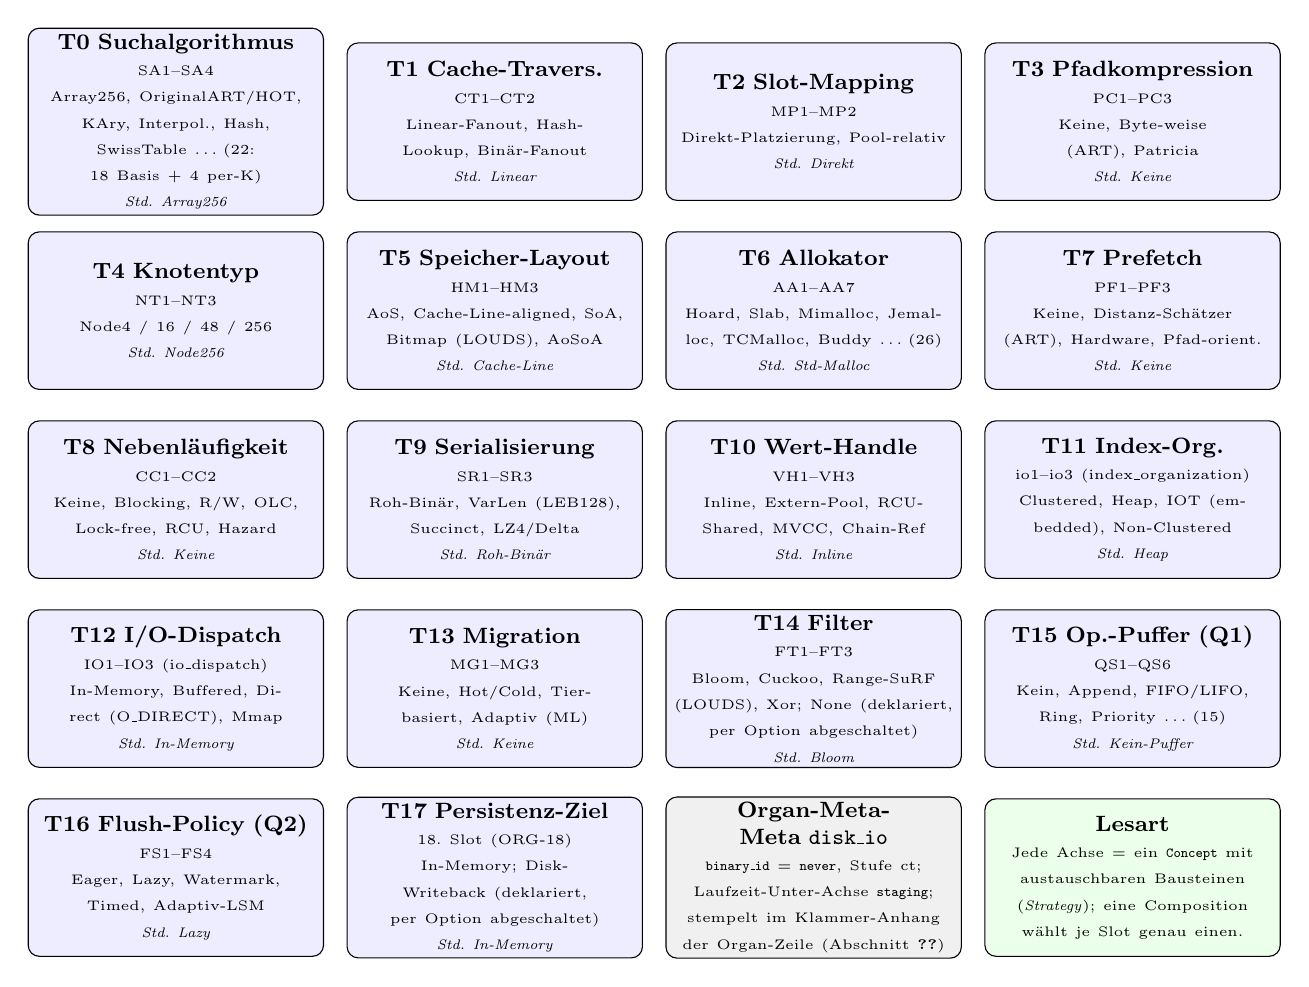
\begin{tikzpicture}[font=\footnotesize,
  ax/.style={draw,rounded corners,fill=blue!7,minimum width=3.75cm,minimum height=2.0cm,text width=3.55cm,align=center,inner sep=2pt}]
  \node[ax] (t0) at (0,0){\textbf{T0 Suchalgorithmus}\\{\tiny SA1--SA4}\\{\tiny Array256, OriginalART/HOT, KAry, Interpol., Hash, SwissTable \dots\,(22: 18 Basis $+$ 4 per-K)}\\{\tiny\itshape Std.\ Array256}};
  \node[ax] (t1) at (4.05,0){\textbf{T1 Cache-Travers.}\\{\tiny CT1--CT2}\\{\tiny Linear-Fanout, Hash-Lookup, Binär-Fanout}\\{\tiny\itshape Std.\ Linear}};
  \node[ax] (t2) at (8.1,0){\textbf{T2 Slot-Mapping}\\{\tiny MP1--MP2}\\{\tiny Direkt-Platzierung, Pool-relativ}\\{\tiny\itshape Std.\ Direkt}};
  \node[ax] (t3) at (12.15,0){\textbf{T3 Pfadkompression}\\{\tiny PC1--PC3}\\{\tiny Keine, Byte-weise (ART), Patricia}\\{\tiny\itshape Std.\ Keine}};
  \node[ax] (t4) at (0,-2.4){\textbf{T4 Knotentyp}\\{\tiny NT1--NT3}\\{\tiny Node4 / 16 / 48 / 256}\\{\tiny\itshape Std.\ Node256}};
  \node[ax] (t5) at (4.05,-2.4){\textbf{T5 Speicher-Layout}\\{\tiny HM1--HM3}\\{\tiny AoS, Cache-Line-aligned, SoA, Bitmap (LOUDS), AoSoA}\\{\tiny\itshape Std.\ Cache-Line}};
  \node[ax] (t6) at (8.1,-2.4){\textbf{T6 Allokator}\\{\tiny AA1--AA7}\\{\tiny Hoard, Slab, Mimalloc, Jemalloc, TCMalloc, Buddy \dots\,(26)}\\{\tiny\itshape Std.\ Std-Malloc}};
  \node[ax] (t7) at (12.15,-2.4){\textbf{T7 Prefetch}\\{\tiny PF1--PF3}\\{\tiny Keine, Distanz-Schätzer (ART), Hardware, Pfad-orient.}\\{\tiny\itshape Std.\ Keine}};
  \node[ax] (t8) at (0,-4.8){\textbf{T8 Nebenläufigkeit}\\{\tiny CC1--CC2}\\{\tiny Keine, Blocking, R/W, OLC, Lock-free, RCU, Hazard}\\{\tiny\itshape Std.\ Keine}};
  \node[ax] (t9) at (4.05,-4.8){\textbf{T9 Serialisierung}\\{\tiny SR1--SR3}\\{\tiny Roh-Binär, VarLen (LEB128), Succinct, LZ4/Delta}\\{\tiny\itshape Std.\ Roh-Binär}};
  \node[ax] (t10) at (8.1,-4.8){\textbf{T10 Wert-Handle}\\{\tiny VH1--VH3}\\{\tiny Inline, Extern-Pool, RCU-Shared, MVCC, Chain-Ref}\\{\tiny\itshape Std.\ Inline}};
  \node[ax] (t11) at (12.15,-4.8){\textbf{T11 Index-Org.}\\{\tiny io1--io3 (index\_organization)}\\{\tiny Clustered, Heap, IOT (embedded), Non-Clustered}\\{\tiny\itshape Std.\ Heap}};
  \node[ax] (t12) at (0,-7.2){\textbf{T12 I/O-Dispatch}\\{\tiny IO1--IO3 (io\_dispatch)}\\{\tiny In-Memory, Buffered, Direct (O\_DIRECT), Mmap}\\{\tiny\itshape Std.\ In-Memory}};
  \node[ax] (t13) at (4.05,-7.2){\textbf{T13 Migration}\\{\tiny MG1--MG3}\\{\tiny Keine, Hot/Cold, Tier-basiert, Adaptiv (ML)}\\{\tiny\itshape Std.\ Keine}};
  \node[ax] (t14) at (8.1,-7.2){\textbf{T14 Filter}\\{\tiny FT1--FT3}\\{\tiny Bloom, Cuckoo, Range-SuRF (LOUDS), Xor; None (deklariert, per Option abgeschaltet)}\\{\tiny\itshape Std.\ Bloom}};
  \node[ax] (t15) at (12.15,-7.2){\textbf{T15 Op.-Puffer (Q1)}\\{\tiny QS1--QS6}\\{\tiny Kein, Append, FIFO/LIFO, Ring, Priority \dots\,(15)}\\{\tiny\itshape Std.\ Kein-Puffer}};
  \node[ax] (t16) at (0,-9.6){\textbf{T16 Flush-Policy (Q2)}\\{\tiny FS1--FS4}\\{\tiny Eager, Lazy, Watermark, Timed, Adaptiv-LSM}\\{\tiny\itshape Std.\ Lazy}};
  \node[ax] (t17) at (4.05,-9.6){\textbf{T17 Persistenz-Ziel}\\{\tiny 18.\ Slot (ORG-18)}\\{\tiny In-Memory; Disk-Writeback (deklariert, per Option abgeschaltet)}\\{\tiny\itshape Std.\ In-Memory}};
  \node[draw,rounded corners,fill=gray!12,minimum width=3.75cm,minimum height=2.0cm,text width=3.55cm,align=center,inner sep=2pt] (mm) at (8.1,-9.6){\textbf{Organ-Meta-Meta \texttt{disk\_io}}\\{\tiny \texttt{binary\_id} $=$ \texttt{never}, Stufe ct; Laufzeit-Unter-Achse \texttt{staging}; stempelt im Klammer-Anhang der Organ-Zeile (Abschnitt~\ref{sec:axis-triad})}};
  \node[draw,rounded corners,fill=green!8,minimum width=3.75cm,minimum height=2.0cm,text width=3.55cm,align=center,inner sep=2pt] (leg) at (12.15,-9.6){\textbf{Lesart}\\{\tiny Jede Achse $=$ ein \texttt{Concept} mit austauschbaren Bausteinen (\emph{Strategy}); eine Composition wählt je Slot genau einen.}};
\end{tikzpicture}
\caption{Galerie der achtzehn Organ-Achsen (T0--T17, kanonische Slot-Reihenfolge): je Achse das Implementierungs-Konzept --- Kurzname, Unter-Achsen-Familie und eine repräsentative Auswahl der austauschbaren Bausteine. Jede Achse ist ein \texttt{Concept}-Interface mit mehreren Strategie-Bausteinen (\emph{Strategy}-Muster); eine konkrete Composition belegt je Slot genau einen. Der \emph{Standard} (\enquote{Std.}) ist eine abgeleitete Vergleichs-Baseline, kein Code-Flag. Die Zahlen in Klammern (T0, T6, T15) sind die \emph{Kataloge} der vollständigen Typlisten (\texttt{All*}); das \emph{Enabled-Inventar} einer Build-Konfiguration ist die vom Enable-Filter gebildete Teilmenge, die die generierte Registry-XML je Achse ausweist (etwa vier Suchalgorithmen und drei Allokatoren im Haus-Default). Die T-Nummern sind Slots der Komposition, keine Verzeichnis-Nummern der Implementierung; die Kürzel io1--io3 und IO1--IO3 gehören zu verschiedenen Achsen (Index-Organisation und I/O-Dispatch). Neben den achtzehn Slots steht die Organ-Meta-Meta \texttt{disk\_io}; das Persistenz-Ziel ist im kanonischen Referenz-Katalog auf seinen In-Memory-Vertreter festgelegt (Abschnitt~\ref{sec:axis-triad}). Die vollständige Matrix mit Herkunfts-Quellen führt Anhang~\ref{app:blocks}.}\label{fig:axes-gallery}
\end{figure}

\subsection{Die eine Architektur im Code}\label{sec:impl-architecture}
Die \emph{eine} Architektur aus Abschnitt~\ref{sec:anatomy-model} ist im Code eine einzige Hierarchie.
Ihre Wurzel ist \texttt{IExecutionEngine} mit drei Engine-Arten --- Anatomy, Virus, Hybrid --- und einem
Vertrag aus sieben Methoden: \texttt{warm\_up}, \texttt{run}, \texttt{reset} und \texttt{shutdown} als
Mess-Lebenszyklus sowie \texttt{engine\_name}, \texttt{engine\_kind} und \texttt{lifecycle\_state} als
Auskünfte. Unter ihr liegen auf Ebene~1 die vier Gattungen Map, Container, Graph und HeuristikAdapter
(Abschnitt~\ref{sec:anatomy-levels}) --- Graph als deklarierter Stub ohne Genus --- und auf Ebene~2 die
sechs Genera SearchAlgorithm, Set, Sequence, Adapter, View und FunctionInterfaceReroute; die Gattung ist im
Code die Ableitung des Genus (\texttt{gattung\_of}), kein zweites Etikett. Das Lebewesen
\texttt{SearchAlgorithm} und seine ABI-Laufzeit-Sicht --- die \enquote{SearchEngine} --- sind zwei
Sichten desselben Gegenstands über die Modulgrenze, kein paralleles Konstrukt: Der Körper ist
\texttt{SearchAlgorithmAnatomy<C>}, die Komposition und Verdrahtung der achtzehn Organe, und die Sicht ist
\texttt{SearchAlgorithmAbiAdapter<A>}, die ihn über die Modulgrenze exportiert. Die Schichtung
\texttt{CacheEngine}\,$\to$\,\texttt{ExecutionEngine}\,$\to$\,\texttt{SearchEngine} (vgl.\ Abschnitt~\ref{sec:repos})
trennt damit Rollen, nicht Klassenbäume: die \texttt{CacheEngine} als Achsen-Bausteine-Bibliothek, die
\texttt{ExecutionEngine} als lebende Wurzel der Ausführungs- und Mess-Werkzeuge (OS-Primitiven; im
Experiment-Modus der Mess-Aggregator über genau eine Beobachter-Schnittstelle) und die
\texttt{SearchEngine} als die über genau diese Schnittstelle vermessene Such-API-Sicht --- das
gleichnamige Bibliotheks-Skelett \texttt{libs/search\_engine} enthält keinen Code
(Abschnitt~\ref{sec:repos}). Achsenlose \emph{Viren} stehen als Geschwister unter derselben Wurzel (im
Bestand eine Graph-Breitensuche), besitzen aber keine Anatomie (Abbildung~\ref{fig:one-architecture}). In
dieser Hierarchie ist der Compiler-Compiler-Charakter des Apparats verankert: Jede Composition ist ein Typ,
aus dem der Builder je Permutation ein eigenes Kompilat erzeugt.

\begin{figure}[!htbp]
  \centering
  %% INTERN-272: KA-063
  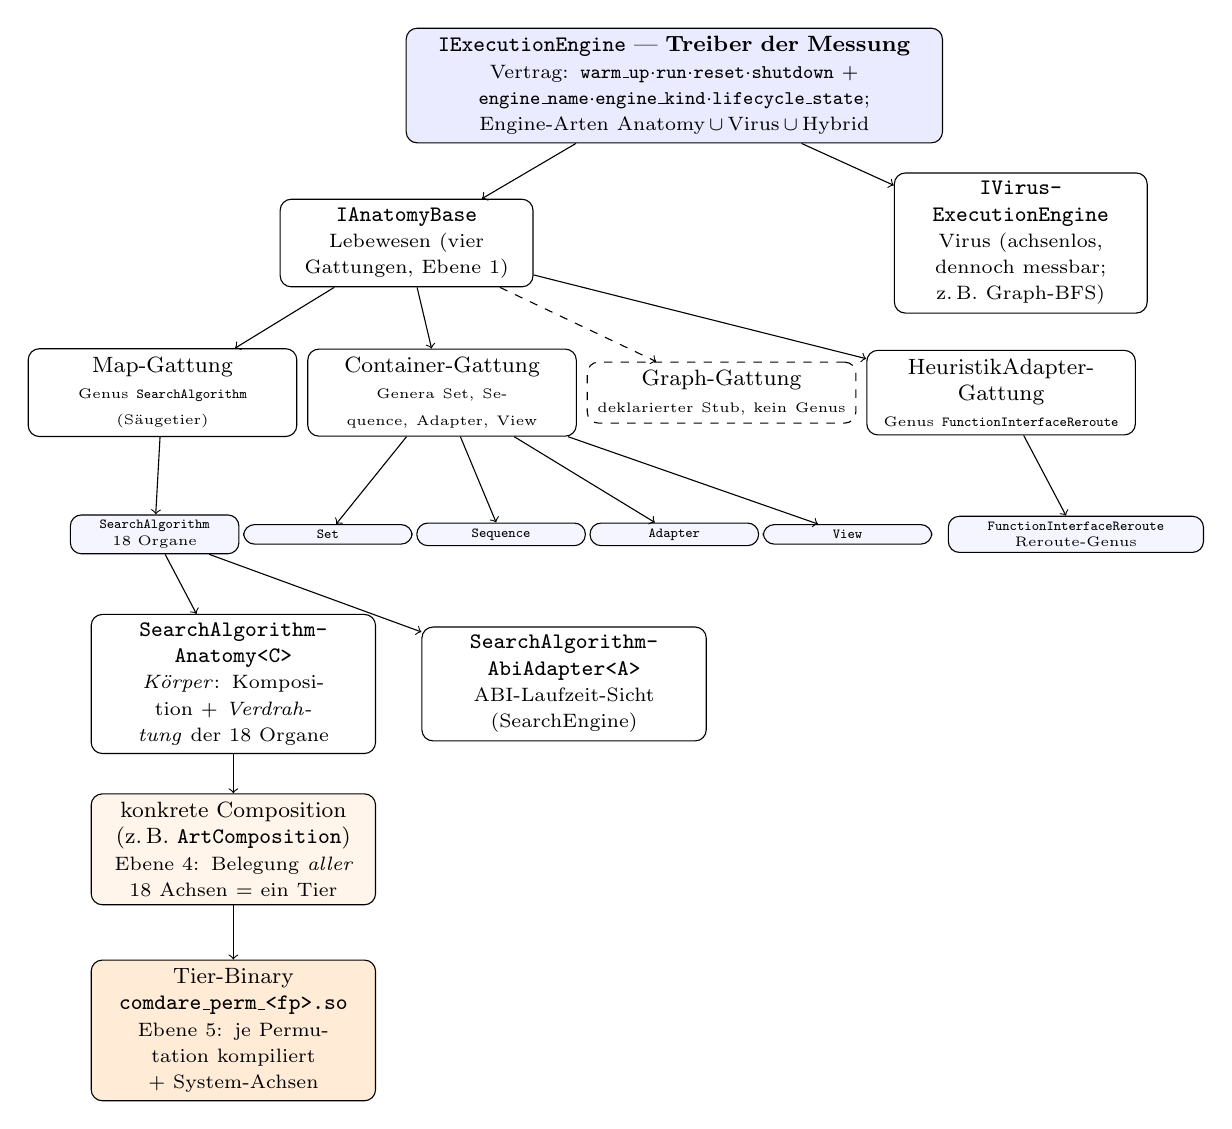
\begin{tikzpicture}[box/.style={draw, rounded corners, align=center, font=\footnotesize, inner sep=3pt, text width=3.0cm},
    gen/.style={draw, rounded corners, align=center, font=\tiny, inner sep=2pt, text width=2.0cm, fill=blue!4}]
    \node[box,fill=blue!8,text width=6.6cm] (root) at (-1.0,0) {\texttt{IExecutionEngine} --- \textbf{Treiber der Messung}\\{\scriptsize Vertrag: \texttt{warm\_up$\cdot$run$\cdot$reset$\cdot$shutdown} $+$ \texttt{engine\_name$\cdot$engine\_kind$\cdot$lifecycle\_state}; Engine-Arten Anatomy\,$\cup$\,Virus\,$\cup$\,Hybrid}};
    \node[box] (ana) at (-4.4,-2.0) {\texttt{IAnatomyBase}\\{\scriptsize Lebewesen (vier Gattungen, Ebene~1)}};
    \node[box] (vir) at (3.4,-2.0) {\texttt{IVirus\-Execution\-Engine}\\{\scriptsize Virus (achsenlos, dennoch messbar; z.\,B.\ Graph-BFS)}};
    \node[box,text width=3.2cm] (g1) at (-7.5,-3.9) {Map-Gattung\\{\tiny Genus \texttt{SearchAlgorithm} (Säugetier)}};
    \node[box,text width=3.2cm] (g2) at (-3.95,-3.9) {Container-Gattung\\{\tiny Genera Set, Sequence, Adapter, View}};
    \node[box,text width=3.2cm,dashed] (g3) at (-0.4,-3.9) {Graph-Gattung\\{\tiny deklarierter Stub, kein Genus}};
    \node[box,text width=3.2cm] (g4) at (3.15,-3.9) {HeuristikAdapter-Gattung\\{\tiny Genus \texttt{FunctionInterfaceReroute}}};
    \node[gen] (n1) at (-7.6,-5.7) {\texttt{SearchAlgorithm}\\18 Organe};
    \node[gen] (n2) at (-5.4,-5.7) {\texttt{Set}};
    \node[gen] (n3) at (-3.2,-5.7) {\texttt{Sequence}};
    \node[gen] (n4) at (-1.0,-5.7) {\texttt{Adapter}};
    \node[gen] (n5) at (1.2,-5.7) {\texttt{View}};
    \node[gen,text width=3.1cm] (n6) at (4.1,-5.7) {\texttt{FunctionInterfaceReroute}\\Reroute-Genus};
    \node[box,text width=3.4cm] (body) at (-6.6,-7.6) {\texttt{Search\-Algorithm\-Anatomy<C>}\\{\scriptsize \emph{Körper}: Komposition $+$ \emph{Verdrahtung} der 18 Organe}};
    \node[box,text width=3.4cm] (abi) at (-2.4,-7.6) {\texttt{Search\-Algorithm\-Abi\-Adapter<A>}\\{\scriptsize ABI-Laufzeit-Sicht (\enquote{SearchEngine})}};
    \node[box,fill=orange!8,text width=3.4cm] (comp) at (-6.6,-9.7) {konkrete Composition (z.\,B.\ \texttt{ArtComposition})\\{\scriptsize Ebene 4: Belegung \emph{aller} 18 Achsen $=$ ein Tier}};
    \node[box,fill=orange!16,text width=3.4cm] (bin) at (-6.6,-12.0) {Tier-Binary \texttt{comdare\_perm\_\-<fp>.so}\\{\scriptsize Ebene 5: je Permutation kompiliert $+$ System-Achsen}};
    \draw[->] (root) -- (ana);
    \draw[->] (root) -- (vir);
    \draw[->] (ana) -- (g1); \draw[->] (ana) -- (g2); \draw[->,dashed] (ana) -- (g3); \draw[->] (ana) -- (g4);
    \draw[->] (g1) -- (n1);
    \draw[->] (g2) -- (n2); \draw[->] (g2) -- (n3); \draw[->] (g2) -- (n4); \draw[->] (g2) -- (n5);
    \draw[->] (g4) -- (n6);
    \draw[->] (n1) -- (body);
    \draw[->] (n1) -- (abi);
    \draw[->] (body) -- (comp);
    \draw[->] (comp) -- (bin);
  \end{tikzpicture}
  \caption{Die \emph{eine} Architektur als einzige Hierarchie ohne Parallel-Bäume. An der Wurzel steht
  \texttt{IExecutionEngine} als \emph{Treiber der Messung} --- der universelle messbare Vertrag aus
  Mess-Lebenszyklus (\texttt{warm\_up}/\texttt{run}/\texttt{reset}/\texttt{shutdown}) und Auskünften
  (\texttt{engine\_name}/\texttt{engine\_kind}/\texttt{lifecycle\_state}) über alle drei Engine-Arten
  Anatomy, Virus und Hybrid; unter ihm verzweigen die anatomie-tragenden \emph{Gattungen} (Ebene~1: Map,
  Container, Graph, HeuristikAdapter) mit ihren \emph{Genera} (Ebene~2) und die achsenlosen \emph{Viren}.
  \texttt{SearchAlgorithm} \emph{ist} das fokale Lebewesen (Säugetier); seine Anatomie ist sein
  \emph{Körper} --- die feste Komposition \emph{und Verdrahtung} der 18 Organe ---, und
  \enquote{SearchEngine} nur dessen ABI-Laufzeit-Sicht. Der Säugetier-Ast ist bis zum Individuum
  ausgezogen: eine konkrete Achsen-Composition (Ebene~4) wird je Permutation als eigenständige Tier-Binary
  kompiliert (Ebene~5). Container besitzt einen eigenen Organsatz mit den Genera Set, Sequence, Adapter und
  View, deren Aritäten die Genus-Bau-Zulassung führt; Graph ist deklariert und besitzt keinen Genus; die
  Gattung HeuristikAdapter führt das Reroute-Genus der Hybrid-Stufe.}\label{fig:one-architecture}
\end{figure}

Konkret ist die Modulgrenze eine C-stabile Schnittstelle --- die ABI (Application Binary Interface) des
Apparats ---, die je Permutation genau ein Lebewesen exportiert (Abbildung~\ref{fig:abi}): Jede Tier-Binary
enthält sieben Pflicht-Symbole mit C-Bindung --- die vier Ur-Symbole ABI-Version, Magic-Zahl, Factory
\texttt{comdare\_\allowbreak{}create\_\allowbreak{}anatomy} und Destroy, dazu die zwei über alle Gattungen
buchstabengleichen Auskünfte \texttt{comdare\_\allowbreak{}anatomy\_\allowbreak{}gattung} und
\texttt{comdare\_\allowbreak{}anatomy\_\allowbreak{}genus} sowie die Versions-Zeilen des Stempels. Die
Buchstabengleichheit ist Bedingung, nicht Bequemlichkeit: Der gattungsunabhängige Loader lädt jede Binary
über dieselbe Ladestrecke (POSIX \texttt{dlopen}~\cite{posix_dlopen}) und kann die Gattung ermitteln,
\emph{bevor} er eine Instanz baut --- gattungsunabhängige Namen mit gattungs-spezifischen Werten; die
Gattung ist dabei aus dem Genus abgeleitet. Die ABI führt die Major-Version~9, deren Naht das
Genus-Interface ist. Die variadische 1/2/N-Hybrid-API gehört zum Prüfling: Seine
\texttt{PrtArtSearchEngine<Ts\ldots>} spezialisiert sich nach Parameterzahl --- ein Parameter fordert alle
Funktionsinterfaces eines \texttt{std::vector}, zwei die eines \texttt{std::map}, mehr als zwei die eines
\texttt{std::map} auf ein Tupel ---, und die Slot-Aritäten der Genera der Cache-Engine (achtzehn für das
Genus SearchAlgorithm, je eigene für Set, Sequence, Adapter und View aus der Genus-Bau-Zulassung) sind
davon getrennt zu lesen. Komplexe Schlüssel reduziert eine Fingerprint-Komponente der Cache-Engine
(\texttt{fixed\_\allowbreak{}length\_\allowbreak{}fingerprint}, FNV-1a-Basis) auf 16-Byte-Binärstrings
fester Länge, die der Prüfling als Schlüsseltyp seines Speichermodells verwendet (\texttt{BinaryKey});
dieser Schlüssel-Fingerprint ist von den drei Identitäts-Fingerprints des Apparats zu unterscheiden ---
dem 64-Bit-Feld \texttt{permutation\_\allowbreak{}fingerprint} im ABI-POD des Moduls, dem
SHA-512-Tier-Fingerprint (Format~6, elf Glieder) und dem SHA-256-Planer-Fingerprint
(Abschnitt~\ref{sec:stamp-model}). Wie diese und die übrigen Code-Interfaces im Detail zusammenhängen,
fasst die UML-Landkarte in Abbildung~\ref{fig:uml-interfaces} zusammen.

\begin{figure}[!htbp]
\begin{lstlisting}[basicstyle=\footnotesize\ttfamily,frame=single,xleftmargin=1.5em]
// C-stabile Modulgrenze: sieben Pflicht-Symbole je Tier-Binary
extern "C" {
  std::uint64_t comdare_anatomy_abi_version();   // ABI-Major 9
  std::uint64_t comdare_anatomy_abi_magic();     // Kompatibilitaets-Probe
  IAnatomyBase* comdare_create_anatomy();        // ein Lebewesen je Permutation
  void          comdare_destroy_anatomy(IAnatomyBase*);
  std::uint8_t  comdare_anatomy_gattung();       // buchstabengleich je Gattung
  std::uint8_t  comdare_anatomy_genus();         // Hybrid: meldet den Ziel-Genus
  AnatomyVersionLines const* comdare_anatomy_version_lines();
}
// Die Hybrid-.so exportiert dieselbe Menge: genau eine Ladestrecke.

// Pruefling-Sicht: variadische 1/2/N-API (Schluessel K, Werte V)
//   1 Parameter  ->  std::vector<V>
//   2 Parameter  ->  std::map<K, V>
//   N > 2        ->  std::map<K, std::tuple<V1, ..., VN>>
template<class K, class First, class... Rest> class PrtArtSearchEngine;
\end{lstlisting}
  \caption{Die ABI-stabile C-Modulgrenze (sieben Pflicht-Symbole; die Hybrid-.so exportiert dieselbe Menge
  und meldet über \texttt{genus} ihr Ziel-Genus) und die variadische 1/2/N-API als Sicht des Prüflings.
  Komplexe Schlüssel reduziert eine Fingerprint-Komponente auf 16-Byte-Binärstrings fester Länge; die
  Identität einer Binary führen davon getrennt das \texttt{permutation\_fingerprint}-Feld des ABI-POD, der
  SHA-512-Tier-Fingerprint und der SHA-256-Planer-Fingerprint.}\label{fig:abi}
\end{figure}

\begin{figure}[htbp]\centering
%% INTERN-272: KA-064
\begin{tikzpicture}[font=\footnotesize,>=Stealth,align=center,
  iface/.style={draw,rounded corners,fill=blue!7,minimum width=4.6cm,minimum height=0.72cm,font=\ttfamily\scriptsize},
  comp/.style={draw,fill=green!8,minimum width=4.6cm,minimum height=0.72cm,font=\ttfamily\scriptsize},
  alt/.style={draw,dashed,gray,minimum width=4.6cm,minimum height=0.72cm,font=\ttfamily\scriptsize,text=gray}]
  \node[font=\bfseries\scriptsize] at (-4.9,5.8){Engine-/Anatomie-Hierarchie};
  \node[iface,minimum height=1.0cm] (exec) at (-4.9,5.05){IExecutionEngine\\{\normalfont\scriptsize Treiber der Messung}};
  \node[iface] (anat) at (-4.9,3.75){IAnatomyBase};
  \node[iface] (virus) at (-0.2,5.05){IVirusExecutionEngine};
  \node[comp] (gatt) at (-4.9,2.75){Gattung (4, Ebene 1)};
  \node[comp] (genus) at (-4.9,1.75){Genus (6, Ebene 2)};
  \node[comp] (body) at (-4.9,0.75){SearchAlgorithmAnatomy<C>};
  \node[comp] (abi) at (-4.9,-0.25){SearchAlgorithmAbiAdapter<A>};
  \node[iface,fill=orange!10] (drive) at (-4.9,-1.35){IDriveableTier / IObservableTier};
  \node[iface,fill=orange!10] (mess) at (-4.9,-2.35){IMessVisitor\\{\normalfont\scriptsize Fläche 3: Mess-Durchstich}};
  \draw[->] (exec)--(anat); \draw[->] (exec.east) to[bend left=10] (virus.west);
  \draw[->] (anat)--(gatt); \draw[->] (gatt)--(genus); \draw[->] (genus)--(body); \draw[->] (body)--(abi); \draw[->] (abi)--(drive); \draw[->] (drive)--(mess);
  \node[font=\bfseries\scriptsize] at (4.9,5.8){Implementierungs-Muster je Achse ($\times$18)};
  \node[iface] (topic) at (4.9,5.05){TopicConcept $\wedge$ AxisConcept};
  \node[comp] (crtp) at (4.9,3.95){AxisBase<Derived> (CRTP)};
  \node[comp] (all) at (4.9,2.85){All*: mp\_list<Baustein$_{1..k}$>};
  \node[comp] (filt) at (4.9,1.75){mp\_filter<is\_enabled>};
  \node[comp] (en) at (4.9,0.65){Enabled*-Liste};
  \node[iface] (slot) at (4.9,-0.45){Composition-Slot (genau ein Typ)};
  \node[alt] (resolve) at (4.9,-1.75){resolve\_baustein<Tag> (verworfen)};
  \draw[->] (topic)--(crtp); \draw[->] (crtp)--(all); \draw[->] (all)--(filt); \draw[->] (filt)--(en); \draw[->] (en)--(slot);
  \draw[->,dashed,gray] (body.east) to[bend right=14] node[midway,below,font=\scriptsize\itshape,text=gray]{komponiert 18 Achsen} (topic.west);
\end{tikzpicture}
\caption{UML-Landkarte der Code-Interfaces: links die Engine-/Anatomie-Hierarchie --- die messbare Wurzel \texttt{IExecutionEngine} als \emph{Treiber der Messung} (Anatomy\,$\cup$\,Virus\,$\cup$\,Hybrid) über \texttt{IAnatomyBase}, den vier Gattungen und sechs Genera und der achsenlosen \texttt{IVirus\-Execution\-Engine}, darunter der \emph{Körper} \texttt{Search\-Algorithm\-Anatomy<C>} (Komposition \emph{und Verdrahtung} der achtzehn Achsen) und seine ABI-Laufzeit-Sicht \texttt{Search\-Algorithm\-Abi\-Adapter<A>} (\enquote{SearchEngine}), die über die Treib-/Beobachter-Verträge \texttt{IDriveableTier}/\texttt{IObservableTier} gemessen wird und deren Messung als Fläche~3 durch den Visitor \texttt{IMessVisitor} quert; rechts der je Achse wiederholte Live-Weg --- ein zweischichtiges \texttt{Concept}, eine \texttt{requires}-gesicherte CRTP-Basis, die vollständige \texttt{mp\_list}-Baustein-Familie, der Übersetzungszeit-Filter über das Enable-Flag und der Composition-Slot, der genau einen Typ enthält. Die variant-basierte Auflösung \texttt{resolve\_baustein} ist eine verworfene, vom Bau isolierte Alternative (gestrichelt).}\label{fig:uml-interfaces}
\end{figure}

\subsection{Vom Profil zur Tier-Binary: Planer, Builder und Mess-Pipeline}\label{sec:impl-pipeline}
Die Kette von der Anwender-XML zur Tier-Binary (Abschnitt~\ref{sec:mess-chain}) hat im Code eine
benannte Gestalt aus zwei Binaries. Stufe~1, die Planer-Rolle, ist \texttt{comdare-experiment-planner}
mit den Subkommandos \texttt{validate}, \texttt{plan dump|ci|cmake}, \texttt{cache-key},
\texttt{fingerprint}, \texttt{status}, \texttt{check-size}, \texttt{simulate}, \texttt{version} und
\texttt{help}. \texttt{validate} prüft rein lesend das per XML-Parser aufgelöste Profil gegen die
einkompilierten Registry-Kataloge (eine unregistrierte Referenz ist ein harter Validierungsfehler,
Abschnitt~\ref{sec:mess-chain}), baut dabei keine Binary und misst nicht. \texttt{plan} fährt den
deterministischen Walk des \texttt{ExperimentPlanDirector} --- nach den Entwurfsmustern \emph{Director}
und \emph{Builder}~\cite{gamma1994patterns} getrennt: Der Director besitzt den \emph{einen}
Enumerations-Walk über Mess-Kombinationen, System-Permutationen und Organ-Schritte, und je Ausgabe-Syntax
(Text-Plan, CI-Pipeline-Beschreibung, CMake-Fragment) emittiert ein konkreter Builder über Hook-Methoden
---; zwei Läufe sind byte-gleich, und der Plan-Kopf annotiert das Registry-Trio der drei Angebots-Kataloge
Organ/System/Mess. \texttt{check-size} und \texttt{simulate} rechnen die Mess-Menge vor dem Lauf aus den
Eingängen des Walks (Abschnitt~\ref{sec:impl-contracts}). Stufe~2, die CEB-Rolle, ist der Mess-Treiber
\texttt{comdare-messung-driver} im Projekt-Repository mit den Subkommandos \texttt{tier ci|cmake},
\texttt{run}, \texttt{version} und \texttt{help}: Er emittiert die Sicht der zweiten Ketten-Stufe ---
System-Permutationen und Tier-Bau-Aufträge seines freigegebenen Bau-Raums --- und fährt den Mess-Lauf;
ein an ihn gerichtetes Planer-Thema beantwortet sein Dispatcher mit dem Verweis auf die Planer-Binary,
statt es still auszuführen. Der Planer steuert die CEB-Aufträge, die CEB steuert die Tier-Aufträge: Die
Rollentrennung ist damit nicht nur Oberfläche, sondern zwei Module. Die emittierten Bau- und
Prüf-Testate halten die Layer-Trennung der Kette sichtbar --- ihre Legenden besitzen drei Formen:
\texttt{ceb:build:[a,b,c]} auf Stufe~1; auf Stufe~2 je Host ein Bau- und Prüf-Batch
\texttt{tier:build-batch:<host>}, dessen Testate je Schritt die getrennte System- und Organ-Klammer
\texttt{zelle=[d,e,f][g,h,i]} enthalten und der die Organ-Bau-Volumina intern in Scheiben zu je 4096 Binaries
bündelt (die Meilenstein-Batches in Abschnitt~\ref{sec:fairness}); und je Host ein Mess-Batch
\texttt{measure:[a,b,c]:batch:<host>}, dessen Mess-Testate als einzige alle drei Klammern
\texttt{zelle=[a,b,c][d,e,f][g,h,i]} enthalten (Abbildung~\ref{fig:traeger-stufen}); die Klammern nennen nur
Haupt-Achsen, Unter-Achsen sind reine Laufzeit-Permutation und stehen in keiner Bau-Legende.

%% INTERN-272: KA-065
Die Anlage hat zwei Steuerpfade: den Planer per Shell direkt und eine API-Kommandozeile mit einem
headless Dienst, der den Planer als Zelle auf Kubernetes oder auf bare metal bedient, sodass eine
vollständige Messreihe ohne interaktive Sitzung angestoßen und beobachtet werden kann. Dazu tritt ein
kommandozeilengeführter Erstellungsmodus für die Anwender-XML mit Hardware-Filter: Nicht verfügbare
Optionen der Zielmaschine sind darin nicht wählbar, und der Modus ist optional --- eine von Hand
geschriebene XML bleibt gleichwertig. Bestand im Code sind die Planer-Hardware-Sonde, die zur Laufzeit den
Host befragt, und die drei Maschinen-Signaturen der System-Registry; Umsetzungsstand: Der Shell-Pfad
ist implementiert; Dienst und Erstellungsmodus sind vorgesehen, aber nicht implementiert.

Zwei Eigenschaften sichern den \emph{einen} Hauptkanal ab. Erstens weist der Text-Plan (Format v1.1) je
Bau-Schritt den tatsächlich erzeugten Datei-Stamm aus (\texttt{built\_stem}) --- erzeugt von \emph{derselben}
Orchestrator-Funktion, die auch der Bau-Orchestrator beim Bau aufruft: Der Plan behauptet keinen
Namen, den der Bau nicht produziert, und ein nicht bestimmbarer Stamm wird als \enquote{-} geschrieben
statt synthetisiert. Zweitens gibt es \emph{eine} XML-Quelle und \emph{einen} Kanal, der sie baut: Die
Variantenbildung liegt in der C++23-Metaprogrammierung, CMake ist auf die Rolle des Bauens beschränkt,
und ein zweiter Emissions-Kanal für Permutations-Quelltexte existiert im Quellbaum nicht.

Innerhalb der CEB überführt der Builder jedes Profil in ein vorkompiliertes C++23-Modul. Jede Permutation
ist durch eine bit-gepackte \emph{Permutations-Flag}-Struktur identifiziert, die zehn Bänke zu je 64~Bit
umfasst (Seitentyp, Knoten, Traversierung, Wert-Handle, Layout, Allokator, Prefetch, Nebenläufigkeit, ISA
und Telemetrie) und hexadezimal serialisiert wird; die Allokator-Unter-Achsen AA1--AA7 führen eine eigene
Flag-Bank. Ein Constraint-Filter der Flag-Struktur (\texttt{is\_valid\_combination}, vier Regeln, etwa:
Leaf-Only-Zähler nur zusammen mit rückwirkender Aggregation) schließt inkohärente Kombinationen aus. Die
achtzehn Organ-Achsen identifiziert der Mess-Pfad über den string-serialisierten Achtzehn-Segment-Pfad
(die \texttt{binary\_id}, Abschnitt~\ref{sec:stamp-model}) samt den drei Fingerprints; die
Permutations-Zählung über die Achsen folgt einer Mixed-Radix-Kodierung, in der jede Achse eine Stelle mit
ihrer eigenen Basis ist --- die Gestalt eines Produktraums, wie ihn die Variabilitätsmodelle der
Software-Produktlinien beschreiben~\cite{pohl2005spl}. Über diese Bausteine läuft die
\emph{Sieben-Phasen-Mess-Pipeline} (Abbildung~\ref{fig:pipeline}) der \texttt{ExperimentDriver}-Bibliothek
je Reihe mit den Phasen des Codes: (1)~\textsc{Enumerate} (XML-Configs parsen, Permutationsliste
aufbauen), (2)~\textsc{Generate} (ein \texttt{comdare\_perm\_<fp>.cpp} je Permutation plus
Aggregator-CMakeLists, dazu \texttt{generate\_\allowbreak{}module\_\allowbreak{}from\_\allowbreak{}profile}
für die SOTA-Profile), (3)~\textsc{Compile} (CMake-Konfiguration und Bau aller Permutations-Module),
(4)~\textsc{Link+Load} (\texttt{dlopen} aller Module), (5)~\textsc{Execute} (\texttt{create\_instance} +
profilbewusstes \texttt{run\_workload}), (6)~\textsc{Measure} (binäre Mess-Records aggregieren) und
(7)~\textsc{Persist} (CSV und JSON, optional binär); zwei opt-in-Phasen kompilieren fehlende Module im laufenden Experiment nach
(\texttt{phase3\_hot\_compile\_missing}) und fahren je Modul einen Funktionstest --- Erzeugen und
Zerstören einer Instanz, ein \texttt{run\_workload} mit leerem Workload-Deskriptor und die Prüfung der
ABI-Version (\texttt{phase4b\_functional\_tests}). Die Messreihen-Modi \texttt{Defined}, \texttt{Full} und
\texttt{FullSampled} (deterministische 1:$n$-Teilmenge des Vollraums, Abschnitt~\ref{sec:mess-chain})
wählen, welche Permutationen eine Reihe umfasst. Die nachgelagerte Auswertungs-Werkzeugkette
(Abbildung~\ref{fig:toolchain}) ist eine Folge von neun numerierten Programmen von
\texttt{sample\_data\_generator} bis \texttt{tex\_formatter}; ihre Ausgabe ist die xlsx-Mappe, der
Standard; die CSV-Form ist kein einzelnes Kind-Dokument, sondern ein geordneter Baum aus CSV-Dateien ---
ein Gesamtordner je Mappe, darunter ein Ordner je Blatt, darin die CSV-Dateien der einzelnen
Unter-Achsen-Fahrten ---, der immer aus der Mappe erzeugt wird (xlsx nach csv, als Strategie derselben
Factory) und per XML statt der Mappe oder zusätzlich zu ihr am selben Ziel liegt (vier registrierte
Rückschreib-Methoden, Abschnitt~\ref{sec:impl-system-axes}). Umsetzungsstand: Die Naht schreibt die
CSV-Projektion als eine flache Datei (\texttt{projektion\_\allowbreak{}oeffnen} in
\texttt{ergebnis\_\allowbreak{}mappe\_\allowbreak{}naht}); die Baumform ist vorgesehen, aber nicht implementiert. Die
Mess-Kopplungen sind über das \texttt{COMDARE\_\allowbreak{}MEASUREMENT\_\allowbreak{}ON}-Gating vom
Produktiv-Pfad getrennt (Abschnitt~\ref{sec:repos}), und Continuous Integration~\cite{fowler2006ci} läuft
über alle vier Repositorien (GitLab CI\@; die Repositorien sind zusätzlich nach GitHub gespiegelt).
\begin{figure}[htbp]\centering
%% INTERN-272: KA-066
\begin{tikzpicture}[font=\footnotesize,>=Stealth,align=center,
  ph/.style={draw,rounded corners,fill=blue!6,minimum width=1.6cm,minimum height=0.85cm},
  hi/.style={draw,rounded corners,fill=orange!18,very thick,minimum width=1.6cm,minimum height=0.85cm},
  opt/.style={draw,rounded corners,dashed,fill=orange!8,minimum width=2.0cm,minimum height=0.65cm,font=\scriptsize},
  pb/.style={draw,rounded corners,fill=orange!16,very thick,minimum width=3.7cm,minimum height=1.05cm,text width=3.5cm,font=\scriptsize}]
  \node[font=\bfseries\scriptsize,anchor=west] at (-0.95,0.95){In-Process-Pfad --- \texttt{ExperimentDriver} (7 Phasen)};
  \node[ph] (p1) at (0,0){\textbf{1}\\Enumerate};
  \node[ph] (p2) at (1.95,0){\textbf{2}\\Generate};
  \node[hi] (p3) at (3.9,0){\textbf{3}\\Compile};
  \node[ph] (p4) at (5.85,0){\textbf{4}\\Link+Load};
  \node[hi] (p5) at (7.8,0){\textbf{5}\\Execute};
  \node[hi] (p6) at (9.75,0){\textbf{6}\\Measure};
  \node[ph] (p7) at (11.7,0){\textbf{7}\\Persist};
  \foreach \a/\b in {p1/p2,p2/p3,p3/p4,p4/p5,p5/p6,p6/p7}{\draw[->,thick] (\a)--(\b);}
  \node[font=\scriptsize,text=orange!60!black] at (3.9,0.66){\textsc{Build}};
  \node[font=\scriptsize,text=orange!60!black] at (8.78,0.66){\textsc{Measure}};
  \node[opt] (o1) at (2.9,-1.4){opt-in:\\Hot-Compile};
  \node[opt] (o2) at (5.4,-1.4){opt-in:\\Funktionstest je Modul};
  \draw[->,dashed] (o1)--(p3);
  \draw[->,dashed] (o2)--(p4);
  \node[font=\bfseries\scriptsize,anchor=west] at (-0.95,-2.5){Out-of-Process-Pfad --- \texttt{BuildOrchestrator} $+$ \texttt{perm\_runner} (Design-Entscheidung)};
  \node[pb] (b1) at (2.0,-3.95){\textbf{build} \texttt{Build\-Orchestrator}: baut \emph{alle} Tier-Binaries zuerst (resumierbar, RAM-gewahr)};
  \node[pb] (b2) at (8.0,-3.95){\textbf{measure} \texttt{perm\_runner}: lädt $+$ misst jede Tier-Binary einzeln (1 DLL/Prozess, via \texttt{IObservableTier})};
  \draw[->,very thick] (b1)--node[above,font=\scriptsize]{Tier-Binaries} (b2);
\end{tikzpicture}
\caption{Die Mess-Pipeline in zwei Ausprägungen. Der \textbf{In-Process-Pfad} (oben) ist die
Sieben-Phasen-Pipeline des \texttt{ExperimentDriver} je Messreihe (Enumerate $\to$ Generate $\to$ Compile
$\to$ Link+Load $\to$ Execute $\to$ Measure $\to$ Persist; zwei opt-in-Phasen kompilieren fehlende Module
im laufenden Experiment nach und fahren je Modul einen Funktionstest mit ABI-Versionsprüfung). Hervorgehoben sind die substanziellen
Phasen: \textsc{Compile} (der \emph{Build} der Tier-Binaries) und \textsc{Execute}/\textsc{Measure} (die
\emph{Messung}); Generate/Link+Load/Persist sind Verdrahtung. Der \textbf{Out-of-Process-Pfad} (unten) ist
eine Design-Entscheidung zur Prozess-Isolation: Der \texttt{BuildOrchestrator} baut \emph{zuerst alle}
Tier-Binaries (resumierbar, RAM-gewahr), danach lädt und misst \texttt{perm\_runner} jede Binary einzeln
über die Beobachter-Schnittstelle \texttt{IObservableTier} --- eine DLL je Prozess, weil die DLL kein
\texttt{main} enthält und der Runner das Executable ist, das sie lädt; kein Zustand wird zwischen
Permutationen geteilt, und eine Cluster-Task fährt genau einen Runner mit genau einer
DLL.}\label{fig:pipeline}
\end{figure}
\begin{figure}[htbp]\centering
%% INTERN-272: KA-067
\begin{tikzpicture}[font=\footnotesize,>=Stealth,align=center,
  tool/.style={draw,rounded corners,fill=blue!6,minimum height=0.7cm,minimum width=3.4cm,inner sep=5pt,font=\ttfamily\scriptsize}]
  \node[tool] (t1) at (0,0){01 sample\_data\_generator};
  \node[tool] (t2) at (4.35,0){02 messung\_driver};
  \node[tool] (t3) at (8.7,0){03 binary\_to\_csv};
  \node[tool] (t4) at (0,-1.5){04 csv\_to\_latex};
  \node[tool] (t5) at (4.35,-1.5){05 diagram\_generator};
  \node[tool] (t6) at (8.7,-1.5){06 latex\_to\_pdf};
  \node[tool] (t7) at (0,-3.0){07 tier\_binary\_report};
  \node[tool] (t8) at (4.35,-3.0){08 appendix\_generator};
  \node[tool] (t9) at (8.7,-3.0){09 tex\_formatter};
  \draw[->,thick] (t1)--(t2);
  \draw[->,thick] (t2)--(t3);
  \draw[->,thick] (t3.south) -- ++(0,-0.4) -- ([yshift=0.4cm]t4.north) -- (t4.north);
  \draw[->,thick] (t4)--(t5);
  \draw[->,thick] (t5)--(t6);
  \draw[->,thick] (t6.south) -- ++(0,-0.4) -- ([yshift=0.4cm]t7.north) -- (t7.north);
  \draw[->,thick] (t7)--(t8);
  \draw[->,thick] (t8)--(t9);
\end{tikzpicture}
\caption[Die nachgelagerte Auswertungs-Werkzeugkette]{Die nachgelagerte Auswertungs-Werkzeugkette als
Neun-Stufen-Kette: \texttt{sample\_data\_generator} erzeugt deterministische Testdaten ohne reale
Hardware, \texttt{messung\_driver} steuert die Messreihen (die CEB-Rolle), \texttt{binary\_to\_csv}
deserialisiert die binären Mess-Records, \texttt{csv\_to\_latex} rendert die booktabs-Tabellen mit einem
Baustein-Steckbrief je Permutations-ID und erzeugt bei leerer Eingabe keine Datei, \texttt{diagram\_generator}
die A4-bewussten TikZ-Diagramme (drei Grund-Plot-Typen Balken, Streudiagramm und Heatmap sowie die darauf
aufbauenden Familien des Mess-Anhangs: ECDF-Treppe, Range-Balken, gestapelte Per-Achsen-Attribution,
Sweep-Kurve, 3D-Rohdaten-Ansicht, Verhältnis-Matrix, normalisierte Balken, Pareto-Streuung und die
Observer-Detail-Tabelle), \texttt{latex\_to\_pdf}
setzt das Manuskript, \texttt{tier\_binary\_report} rastert je Tier-Binary den Interface-Vertrag gegen die
geplante Menge des Text-Plans, \texttt{appendix\_generator} erzeugt als In-Process-Fassade je Sprache die
Kern- und Darstellungs-Dateien des Mess-Anhangs aus \emph{einer} WIDE-Matrix, und \texttt{tex\_formatter}
normalisiert die erzeugten Dateien. Die Ausgabe der Kette ist die xlsx-Mappe; die CSV-Form ist kein
einzelnes Kind-Dokument, sondern der aus der Mappe erzeugte, geordnete Baum aus CSV-Dateien (ein Ordner je
Blatt), im Code als eine flache Datei geschrieben (die Baumform ist vorgesehen, aber nicht implementiert;
Abschnitt~\ref{sec:impl-system-axes}).}\label{fig:toolchain}
\end{figure}

Die Ebenen E4--E0 aus Abschnitt~\ref{sec:anatomy-layers} haben im Code je einen Ort, und die Grenzen
zwischen ihnen besitzen je einen Contract-Test (Abschnitt~\ref{sec:impl-contracts});
Abbildung~\ref{fig:impl-layers} zeigt diese Code-Gestalt, ohne die Ebenen neu zu erklären. E4, die
Definitions- und Auswertungs-Schicht, ist das XML-Profil mit dem Planer
(\texttt{profile\_\allowbreak{}facade/\allowbreak{}planner}) und den Auswertungs-Programmen 04 und 08 der
Werkzeugkette; E3, der Permutations-B\textsuperscript{+}-Baum, ist der Experiment-Baum
(\texttt{experiment\_tree}) mit der \texttt{binary\_id} als Pfad; E2, die Tier-Binaries, sind der
ABI-Adapter mit der Modul-ABI-Deklaration; E1, die Laufzeit-Konfiguration, ist das Interface
\texttt{IResourceControllableTier} zusammen mit den dynamischen Dimensionen der Mess-Registry-XML\@; E0, die
Infrastruktur, sind CI, Runner und Lager; der Querschnitt~M ist die System-Achsen-Wurzel
\texttt{SystemAxis} (Abschnitt~\ref{sec:impl-system-axes}).
\begin{figure}[htbp]\centering
%% INTERN-272: KA-068
\begin{tikzpicture}[font=\footnotesize,>=Stealth,
  eb/.style={draw,rounded corners,fill=blue!7,minimum width=11.4cm,minimum height=0.95cm,text width=11.1cm,align=left,inner sep=3pt},
  ct/.style={font=\tiny,fill=white,inner sep=1pt}]
  \node[eb] (e4) at (0,0){\textbf{E4} Definitions-/Auswertungs-Schicht --- {\scriptsize XML-Profil $+$ Planer (\texttt{profile\_facade/planner}); Auswertung: Programme 04 und 08}};
  \node[eb] (e3) at (0,-1.55){\textbf{E3} Permutations-B$^+$-Baum --- {\scriptsize \texttt{experiment\_tree}; Pfad $=$ \texttt{binary\_id} (18 Segmente, mixed-radix)}};
  \node[eb] (e2) at (0,-3.1){\textbf{E2} Tier-Binaries --- {\scriptsize \texttt{SearchAlgorithmAbiAdapter<A>} $+$ Modul-ABI-Deklaration (sieben Pflicht-Symbole)}};
  \node[eb] (e1) at (0,-4.65){\textbf{E1} Laufzeit-Konfiguration --- {\scriptsize \texttt{IResourceControllableTier} $+$ dynamische Dimensionen der Mess-Registry-XML}};
  \node[eb,fill=gray!12] (e0) at (0,-6.2){\textbf{E0} Infrastruktur --- {\scriptsize CI (vier Repositorien), Runner, Lager}};
  \draw[->,thick] (e4)--(e3); \draw[->,thick] (e3)--(e2); \draw[->,thick] (e2)--(e1); \draw[->,thick] (e1)--(e0);
  \node[ct] at (0,-0.775){\texttt{test\_e4\_contract\_xml\_to\_axislevels} (Fake-E3)};
  \node[ct] at (0,-2.325){\texttt{test\_e3\_contract\_binary\_id\_bijektion} $+$ \texttt{\ldots\_conformance\_gate\_wirksam} (Fake-E2)};
  \node[ct] at (0,-3.875){\texttt{test\_e2\_contract\_abi\_vertrag} (Wormhole-Referenz-DLL, Fake-E1)};
  \node[ct] at (0,-5.425){\texttt{test\_e1\_contract\_rc\_konsum} (in-process, T6/T8/T1/T11)};
  \node[draw,rounded corners,fill=orange!12,minimum width=2.8cm,minimum height=7.15cm,text width=2.6cm,align=center,inner sep=3pt] (m) at (7.3,-3.1){\textbf{M} Mess-Querschnitt\\[3pt]{\scriptsize \texttt{SystemAxis}-Wurzel, host-seitig; berührt keine Binary-Identität}\\[3pt]{\tiny \texttt{test\_m\_\allowbreak contract\_\allowbreak system\_\allowbreak axis\_\allowbreak wurzel}, \texttt{test\_b3\_\allowbreak wallclock\_\allowbreak erbe\_ct}}};
\end{tikzpicture}
\caption[Die Ebenen E4--E0 im Code]{Die Ebenen E4--E0 des Schichtenmodells (Abschnitt~\ref{sec:anatomy-layers}) an ihrem Ort im Code,
mit dem Contract-Test je Grenze (Fake der Nachbar-Ebene) und dem Mess-Querschnitt~M, der alle Ebenen
host-seitig quert, ohne die Binary-Identität zu berühren.}\label{fig:impl-layers}
\end{figure}

Die Verträge zwischen den Träger-Stufen sind an den Binaries in Flächen zergliedert. Das
Drei-Flächen-Modell (Abschnitt~\ref{sec:anatomy-levels}) ist im Code namentlich vorhanden: Fläche~1 ist
das Genus-Interface der Tier-Binary (Laufzeit, Abstract Factory), Fläche~2 der Stempel (Übersetzungszeit,
ABI-stabil) und Fläche~3 der Mess-Durchstich \texttt{IMessVisitor} --- ein Visitor am
\texttt{dlopen}-Übergang mit doppeltem Dispatch, der existiert, \emph{damit} Gattungs- und Genus-Interfaces
unverändert bleiben: Die Messung quert als eigene Naht, statt Mess-Felder in die fachlichen Interfaces zu
drängen. Der Stempel-Vertrag ist als Matrix aus sieben Interfaces und vier Trägern ausgeführt --- 28~Zellen
mit dreiwertiger Zulassung (Pflicht, Erlaubt, Verboten), von denen der Bestand nur Pflicht und Verboten
belegt (Tabelle~\ref{tab:stempel-matrix}): Die statische Selbst-Version führt nur der Planer; Mess- und
System-Zeile führen CEB, Tier und Hybrid; die Organ-Zeile führen nur Tier und Hybrid --- die Absenz beim
CEB ist die statische Sperre \enquote{der CEB führt keine Organ-Achsen} ---; Fingerprint und
Gesamt-Stempel führen alle vier, und die angeschlossenen Stempel-Zeilen führt nur der Hybrid als
Laufzeit-Haken. Geprüft wird der Vertrag nicht in der Basis, sondern unter jeder Erbin: Die Basis ist
leer, und erst ein \texttt{static\_assert(StempelVertrag<Erbin, Traeger>)} direkt unter der Definition
macht eine unparsbare Zeile, eine fehlende Pflicht oder ein verbotenes Interface zum Übersetzungsfehler
--- eine Form des Consumer-Driven Contract~\cite{robinson2006cdc}, in der die Erwartung des konsumierenden
Trägers den Vertrag treibt.
\begin{table}[htbp]\centering\footnotesize
\begin{tabular}{@{}llcccc@{}}
\toprule
Interface & Inhalt & Planer & CEB & Tier & Hybrid \\
\midrule
\texttt{VersionXyz}     & statische Selbst-Version X.Y.Z[.flag]            & P & V & V & V \\
\texttt{MessZeile}      & Stempel-Zeile des Mess-Realms                     & V & P & P & P \\
\texttt{SystemZeile}    & Stempel-Zeile des System-Realms                   & V & P & P & P \\
\texttt{OrganZeile}     & Stempel-Zeile des Organ-Realms                    & V & V & P & P \\
\texttt{FingerprintSha} & Fingerprint-Hex (Planer SHA-256, sonst SHA-512)   & P & P & P & P \\
\texttt{GesamtStempel}  & das eine Kompositum der Erbin                     & P & P & P & P \\
\texttt{Angeschlossene} & angeschlossene Stempel-Zeilen (Laufzeit-Haken)    & V & V & V & P \\
\bottomrule
\end{tabular}
\caption{Der Stempel-Vertrag als Matrix aus sieben Interfaces und vier Trägern (28 Zellen, dreiwertige
Zulassung P = Pflicht, E = Erlaubt, V = Verboten; E ist im Bestand unbelegt). Die Verbots-Zelle der
Organ-Zeile beim CEB ist die statische Sperre \enquote{der CEB führt keine Organ-Achsen}; die Zellen
werden je Erbin per \texttt{static\_assert} geprüft.}\label{tab:stempel-matrix}
\end{table}

\section{Qualitätssicherung: Contract-Tests je Schicht}\label{sec:impl-contracts}
Das Schichtenmodell E4--E0 mit seinen festgeschriebenen Interface-Verträgen hat
Abschnitt~\ref{sec:anatomy-layers} als Konzept entwickelt; dieser Abschnitt beschreibt seine Umsetzung
als Prüf-Infrastruktur. Der Grund liegt in der Schichtung selbst: Änderungen, die mehrere Schichten
zugleich verändern, erzeugen Fehler aus Wechselwirkungen zwischen den Ebenen, die weder lokale Tests
noch zeilenweises Review sichtbar machen (ADR-5, Anhang~\ref{app:adr}). Für ein System, dessen
Produktraum jede vollständige Materialisierung ausschließt (Abschnitt~\ref{sec:mess-chain}), sind
Änderungen über mehrere Ebenen zugleich damit praktisch nicht abnehmbar; die Konsequenz ist, jede Schicht einzeln
fertigzustellen --- mit explizit festgeschriebenem Interface-Vertrag zur Nachbar-Ebene, eigenem
Test-Harness und eigener Abnahme-Definition.

Das tragende Prüfprinzip lautet: \emph{Jede Schicht wird gegen einen übersetzungszeitlichen Ersatz
ihrer Nachbar-Ebene getestet.} Die Contract-Tests sind gewöhnliche Testziele der Build-Pipeline; die
Nachbar-Ebene ersetzt dabei je ein \emph{Fake} --- eine Template- und Concept-basierte Attrappe im
Test-Scope, kein Laufzeit-Umschalter im Produktiv-Code. So kann eine Schicht fertig und abgenommen
sein, bevor die tiefere Ebene ihre Werte überhaupt konsumiert, und die Prüffrage jeder Grenze ---
reicht die Schicht ihre Definition \emph{verlustfrei} an die nächste weiter?
(Abschnitt~\ref{sec:anatomy-layers}) --- wird vom Entwurfsgrundsatz zum ausführbaren Abnahme-Test.

Je Schicht konkretisiert sich das so (Abbildung~\ref{fig:impl-layers}): Für die Definitions- und
Auswertungs-Schicht~E4 prüft der Harness
(\texttt{test\_\allowbreak{}e4\_\allowbreak{}contract\_\allowbreak{}xml\_\allowbreak{}to\_\allowbreak{}axislevels})
die Übersetzung der deklarativen XML-Profile in die Achsen-Ebenen-Struktur --- Golden-Fixtures
vergleichen die aus einem Profil emittierten Achsen-Ebenen strukturell gegen eine erwartete Referenz,
wobei ein Fake-E3 den Permutationsbaum ersetzt; weder Baum-Aufbau noch Bau-Aufträge sind nötig, um die
Grenze E4$\to$E3 abzunehmen. Für den Permutations-B\textsuperscript{+}-Baum~E3 prüft der Harness
(\texttt{test\_\allowbreak{}e3\_\allowbreak{}contract\_\allowbreak{}binary\_\allowbreak{}id\_\allowbreak{}bijektion})
die Bijektion der Binary-Identität: Aus Achsen-Ebenen-Fixtures wird die Permutations-Enumeration gefahren
und je Pfad der mixed-radix-kodierte Binary-Identifier hin- und zurückübersetzt (Zählung plus
Signatur-Roundtrip) --- gegen ein Fake-E2, das keine einzige Binary baut; dazu tritt ein Konformitäts-Gate
im Voll-Lauf-Pfad
(\texttt{test\_\allowbreak{}e3\_\allowbreak{}contract\_\allowbreak{}conformance\_\allowbreak{}gate\_\allowbreak{}wirksam}),
das jede importierte Binary vor der Messung gegen den festgeschriebenen Vertrag prüft. Für die
Tier-Binaries~E2 ist der Vertrag die ABI selbst
(\texttt{test\_\allowbreak{}e2\_\allowbreak{}contract\_\allowbreak{}abi\_\allowbreak{}vertrag}): Die
Wormhole-Referenz-DLL wird geladen und muss die festgeschriebene Schnittstellen-Folge erfüllen ---
\texttt{IAnatomyBase}, \texttt{IObservableTier} und \texttt{IResourceControllableTier} (an jedem Adapter
vorhanden) samt fester Fähigkeits-Auskunft. Die Antwort einer Stellgrößen-Anfrage (\texttt{apply}) ist
dabei kein Fehlercode, sondern die \emph{Zahl der Achsen, die den Wert tatsächlich angenommen haben}: Eine
Anfrage oberhalb der gemeldeten Fähigkeiten wird sichtbar, weil diese Zahl unter der Zahl der angefragten
Achsen bleibt --- im Wormhole-Piloten nehmen von fünf steuerbaren Achsen genau zwei (Batch-Größe und
Inline-Schwelle) den Wert tatsächlich an, ein Nullzeiger liefert null ---, und das ist die
Vollständigkeitsregel der Stellgrößen: Nichts wird still angenommen, jede Rückmeldung zählt nur den
realen Konsum. Das zugehörige Fake-E1 legt die Laufzeit-Stellgrößen an und appliziert sie, verlangt aber
keine Konsum-Wirkung --- die gehört zur Abnahme von E1. Für die Laufzeit-Konfiguration~E1 schließlich
prüfen Edge-Tests (\texttt{test\_\allowbreak{}e1\_\allowbreak{}contract\_\allowbreak{}rc\_\allowbreak{}konsum},
in-process über die Achsen T6, T8, T1 und T11) die Randfälle des dynamischen Regimes: dass ein
wiederverwendetes Tier zwischen zwei Läufen vollständig zurückgesetzt wird, dass ein Pool-Budget
unterhalb des lebenden Datenbestands als benannter Zustand behandelt statt still verletzt wird und dass
jede applizierte Stellgröße als benannte Spalte in der persistierten Ergebnis-Datei sichtbar ist, dazu der
Erhalt der Zwei-Phasen-Operationsschleife (verworfener Warmlauf, Messlauf) als Invariante.
%% INTERN-272: KA-069
Geprüft wird die Persistenz an der Ergebnis-Datei, nicht am In-Process-Zustand; Führung ist dabei die
Standard-xlsx --- die Rückschreib-Registry führt sie als vierte Methode und Default-Auswerteformat, der
xlsx-Writer liegt in der Lager-Ablage ---, und die CSV-Form ist kein einzelnes Kind-Dokument, sondern ein
geordneter Baum aus CSV-Dateien (ein Gesamtordner je Mappe, darunter ein Ordner je Blatt, darin die
CSV-Dateien der einzelnen Unter-Achsen-Fahrten), der immer aus der Mappe erzeugt wird und per XML statt
der Mappe oder zusätzlich zu ihr am selben Ziel liegt. Umsetzungsstand: Die E1-Prüfung liest die
CSV-Ausgabe der Persist-Phase, die die Naht als eine flache Datei schreibt
(\texttt{projektion\_\allowbreak{}oeffnen}); die Prüfung an der je Binary erzeugten xlsx und die Baumform
der CSV-Ablage sind vorgesehen, aber nicht implementiert.

Oberhalb der Schicht-Harnesse sichert ein \emph{Zwei-Gate-Protokoll} jedes Implementierungs-Paket ab.
Sein Zweck ist die Trennung zweier Fragen: Gate~1 sichert das Engine-Repository gegen sich selbst --- die
Einheits- und Vertrags-Tests ---, Gate~2 sichert die Integration in das Projekt-Repository, in dem die
Kette XML $\to$ Binaries $\to$ Messung $\to$ Anhang tatsächlich läuft; erst beide zusammen weisen nach, dass ein
Paket den Apparat nicht bricht (Continuous Integration und Delivery als
Sicherungsstufen~\cite{fowler2006ci,humble2010cd}).
%% INTERN-272: KA-070
\emph{Gate~1} ist das scharfe Gate des Engine-Repositories: Die volle Test-Suite\footnote{Umfang der Test-Suite: 551 registrierte Tests (\texttt{ctest -N}) im
  gcc-Release-Baubaum vom 17.~September 2026.} läuft in vier Zellen, gcc und clang jeweils als
Release- und Debug-Bau, ohne Änderungs-Skip, und akzeptiert wird nur ein Lauf ohne fehlgeschlagene Tests, ohne
Ausnahmeliste. Der Doppellauf hat zwei Gründe: Die Compiler-Matrix zwingt jede statische Prüfung
durch zwei Übersetzer, und die Wiederholung des Messlaufs --- die Zwei-Phasen-Operationsschleife aus
verworfenem Warmlauf und Messlauf im Ein-Thread-deterministischen Modus \texttt{measure} --- macht die
Run-to-Run-Stabilität der Zahl selbst zum Prüfgegenstand. Bestandteil von Gate~1 ist die
Golden-Verankerung des Permutationsraums, und hier sind zwei Begriffe zu trennen
(Abschnitt~\ref{sec:mess-chain}):
%% INTERN-272: KA-071
Der \emph{Referenz-Katalog} des Golden-Tests hält $2^{17} = 131072$ Binary-Identitäten --- siebzehn Achsen
mit je zwei Vertretern, das Persistenz-Ziel auf einen festgelegt --- und wird gegen eine festgeschriebene
CRC-64-Prüfsumme bestätigt (\texttt{0x56F1B721C72DC10E}, CRC-64/ECMA-182 über die Identitäten in % chktex 29
kanonischer Reihenfolge; die Referenz ist literaler Werkzeug-Output, und ihre Änderung ist nur im
Rahmen einer koordinierten Schnittstellen-Änderung zulässig), während ein kleiner, materialisierbarer Katalog von
$4\cdot4\cdot5\cdot4 = 320$ Identitäten als byte-genaue Prüfung der Serialisierungsform dient --- ein
Charakterisierungs-Test im Sinne von Feathers~\cite{feathers2004legacy}, der eine festgeschriebene
Kardinalität als Regressions-Detektor nutzt. Die \emph{Mächtigkeit} des in einer vollständigen Messreihe geplanten Raums
ist davon verschieden und nie statisch: Der Planer zählt sie je Achse aus den in der XML deklarierten
Möglichkeiten im Director-Walk (\texttt{check-size}, \texttt{simulate}) und multipliziert die Stufen über
alle Achsen; sie unterscheidet sich je Plattform durch fehlende Freigaben, und jede Zahl der Rechnung
kommt als Eingang herein, nie als Konstante.
%% INTERN-272: KA-073
\emph{Gate~2} ist das Integrations-Gate des Projekt-Repositories: Seine Pipeline baut fehlerfrei ohne
Ausnahmemenge --- die Regel dieser Arbeit kennt keine geduldeten fehlschlagenden Tests; die beiden deklarierten
Fehlschlag-Duldungen der Messmaschinen liegen im Engine-Repository und sind eine Plattform-Grenze (ein
arm64-Smoke-Bau ohne verfügbaren Runner) und ein manueller Relock-Wartungsjob (er darf nicht ausgeführt
bleiben), keine Testmenge.

Dieses Protokoll ist Methodik, kein Systembestandteil: Es beschreibt, \emph{wie} Änderungen am
Apparat abgenommen werden, nicht, was die Binaries enthalten. Die Verzeichnis- und Suite-Struktur,
auf der es läuft, dokumentiert Anhang~\ref{app:code}.

%% INTERN-272: KA-074
Die Fertigstellung folgt der Schichtung top-down --- E4, E3, E2, dann der Mess-Querschnitt~M
unmittelbar vor E1 ---, und die Infrastruktur~E0 bildet den letzten Schritt der Konsolidierung
(Abschnitt~\ref{sec:anatomy-layers}). Der Reifegrad ist am Test-Bestand ablesbar: Alle vier Grenzen besitzen
ihren Harness (oben), und der Querschnitt~M besitzt einen eigenen, der ohne jede Tier-Binary auskommt
(\texttt{test\_\allowbreak{}m\_\allowbreak{}contract\_\allowbreak{}system\_\allowbreak{}axis\_\allowbreak{}wurzel}
für die System-Achsen-Wurzel und die Mess-Visitierbarkeit,
\texttt{test\_\allowbreak{}b3\_\allowbreak{}wallclock\_\allowbreak{}erbe\_\allowbreak{}ct} für das
Wallclock-Erbe): Eine synthetische Mess-Quelle wird über die System-Achsen-Wurzel getrieben und ihre
Werte bis in die Ergebnis-Spalten verfolgt. Die Mess-Achse treibt dabei die Freigabe der Mess-Quelle über
die System-Achsen-Wurzel in Gestalt der CEB\@: Der Planer delegiert an das CEB-Interface, welche
Binary-Rekombination gegen welche Lasten zu messen ist, und die CEB gibt die Quelle frei.
Umsetzungsstand: Die Hardware-Erhebungskette läuft an der Freigabe-Naht des Builders
(Abschnitt~\ref{sec:impl-system-axes}); der CEB-getriebene Freigabe-Pfad der Mess-Quelle ist
vorgesehen, aber nicht implementiert. Die Code-Gestalt des Querschnitts beschreibt der folgende Abschnitt.

\section{Realm-Wurzeln im Code: System- und Mess-Achsen}\label{sec:impl-system-axes}
%% INTERN-272: KA-075
Vier Abstraktionsebenen ordnen die Begriffe dieses Abschnitts (Abbildung~\ref{fig:m0-m3}), in Anlehnung an
die vierstufige Meta-Ebenen-Architektur der Object Management Group (MOF)~\cite{omg2016mof}, in der M0 die
Laufzeit-Instanzen, M1 das Modell, M2 das Metamodell und M3 das Meta-Metamodell bezeichnet: M3 sind die
\emph{Meta-Meta-Achsen} im Sinne der Indirektion einer Beschreibung --- eine Achse, die beschreibt, wie
andere Achsen beschrieben werden (die Mess-Meta-Meta \texttt{load\_framework}, die Organ-Meta-Meta
\texttt{disk\_io}, die System-Meta-Metas unter dem Hub der Erweiterungs-Hardware); M2 sind als Lesart
die \emph{Meta-Achsen}, die literale Klassifizierung der unter ihrem Begriff geführten Haupt- und
Unter-Achsen --- im Code die Registry-Zeile mit Kategorie, Familie und Bausteinliste; M1 sind Konzeption
und Laufzeit-Implementierung der Haupt- und Unter-Achsen --- die CRTP-Achse mit ihrem Concept; M0 ist der
Binärcode --- die Tier-Binary, in der genau eine Belegung einkompiliert ist. Im Stempel ist die
Meta-Meta-Ebene eines Eintrags mechanisch seine Klammer-Tiefe: Die Bits~3--5 eines Eintrags kodieren die
Ebene, eine Haupt-Achse ist klammerlos, eine Meta-Meta hängt als Klammer-Anhang an ihrer Zeile, und eine
Tiefe über sieben bricht mit Fehlermeldung ab; der Renderer der Meta-Meta-Einträge ist zugleich der Engpass, an dem zwei
Versionsprüfungen jedes gestempelte Glied prüfen, sodass keine neue Meta-Meta diese Prüfung umgehen
kann. Die Kurzform \texttt{c\{p.e\}} eines Versions-Flags bezeichnet dabei \texttt{c} mit den
Untergliedern \texttt{p} und \texttt{e}, nie ein flaches Kürzel. Je Realm gibt es einen eigenen
Meta-Meta-Diskriminator (\texttt{measurement\_meta\_meta}, \texttt{system\_meta\_meta},
\texttt{organ\_meta\_meta}); die PMC-Erfassung --- Performance Monitoring Counter, die Hardware-Zähler der
CPU --- ist eine Meta-Meta-Mess-Achse, weil sie beschreibt, mit welchem Zähler-Instrument andere
Messungen erhoben werden.
\begin{figure}[htbp]\centering
%% INTERN-272: KA-076
\begin{tikzpicture}[font=\footnotesize,>=Stealth,
  mb/.style={draw,rounded corners,minimum width=13.6cm,minimum height=1.05cm,text width=13.3cm,align=left,inner sep=3pt}]
  \node[mb,fill=orange!14] (m3) at (0,0){\textbf{M3 Meta-Meta-Achsen} --- Indirektion einer Beschreibung\\{\scriptsize Beispiele: \texttt{load\_framework} (Mess-Realm, Token \texttt{ycsb@1.0.0.c}), \texttt{disk\_io} (Organ-Realm, Klammer-Anhang), System-Meta-Metas unter \texttt{external\_utils}}};
  \node[mb,fill=orange!8] (m2) at (0,-1.5){\textbf{M2 Meta-Achsen} (Lesart) --- literale Klassifizierung der Haupt- und Unter-Achsen\\{\scriptsize Beispiel: die Registry-Zeile \texttt{<axis id=allocator slot=T06 category=composition \ldots>} mit ihrer Bausteinliste}};
  \node[mb,fill=blue!7] (m1) at (0,-3.0){\textbf{M1 Konzeption und Laufzeit-Implementierung} --- Haupt- und Unter-Achsen\\{\scriptsize Beispiel: die CRTP-Achse \texttt{AxisBase<Derived>} mit ihrem Concept und ihren Bausteinen (Strategy)}};
  \node[mb,fill=gray!12] (m0) at (0,-4.5){\textbf{M0 Binärcode} --- die Tier-Binary\\{\scriptsize Beispiel: \texttt{comdare\_perm\_<fp>.so} mit genau einer einkompilierten Belegung; Identität \texttt{binary\_id} $+$ Fingerprint}};
  \draw[->,thick] (m3)--node[right,font=\tiny]{beschreibt}(m2);
  \draw[->,thick] (m2)--node[right,font=\tiny]{klassifiziert}(m1);
  \draw[->,thick] (m1)--node[right,font=\tiny]{kompiliert zu}(m0);
\end{tikzpicture}
\caption[Die vier Abstraktionsebenen M0--M3]{Die vier Abstraktionsebenen M0--M3 als Lesart der Achsen-Begriffe, in Anlehnung an die
Meta-Ebenen-Architektur der MOF\@: Meta-Meta-Achsen (M3) beschreiben, wie andere Achsen beschrieben
werden; die Registry-Zeile (M2) klassifiziert Haupt- und Unter-Achsen; die CRTP-Achse (M1) ist ihre
Konzeption und Laufzeit-Implementierung; die Tier-Binary (M0) ist der Binärcode genau einer
Belegung.}\label{fig:m0-m3}
\end{figure}

Die Dreiteilung der Achsen-Realms (Abschnitt~\ref{sec:axis-triad}) ist im Code als Typ-Trennung
ausgeführt. Alle Achsen teilen ein gemeinsames Familiendach --- \texttt{topics::Axis<Derived>}, eine
leere, nicht-polymorphe CRTP-Basis, deren Concept-Prüfung (\texttt{is\_empty} und nicht
\texttt{is\_polymorphic}) jede eingeschleppte vtable schon beim Übersetzen zurückweist --- und
deklarieren ihre Kategorie über die Trichotomie \texttt{AxisCategory} und ihre Familie über den
Diskriminator \texttt{AxisKind} mit sechs Werten (Abschnitt~\ref{sec:axes-impl}). Je Familie existiert
eine eigene CRTP-Wurzel: \texttt{OrganAxis} und \texttt{OrganMetaMetaAxis} für den Organ-Realm,
\texttt{SystemAxis} für die Mess-System-Achsen des host-seitigen Querschnitts, \texttt{CebSystemAxis} für
die Bau- und Steuer-Achsen der CEB-Konfiguration, \texttt{SystemMetaMetaAxis} für die System-Meta-Achsen
unter dem Erweiterungs-Hub und \texttt{MeasurementMetaMetaAxis} für die Mess-Realm-Achsen des Planers.
Eine Achse \emph{ist} ihre Familie durch ihre Basisklasse, nicht durch ein umhängbares Etikett ---
\texttt{CebSystemAxis} liefert ihre Art \texttt{axis\_kind()} als harten Rückgabewert
\texttt{system\_config}, weshalb der Mess-Realm eine eigene Wurzel besitzt statt einer wiederverwendeten:
Der System-Realm wurzelt an der CEB, der Mess-Realm am Planer (Abschnitt~\ref{sec:axis-triad}).

%% INTERN-272: KA-077
Auf der System-Seite ist die kanonische Ordnung selbst Code: Das konstante Drei-Element-Array
\texttt{kSystemAxisOrder} hält die System-Haupt-Achsen \texttt{target\_isa}, \texttt{operating\_system} und
\texttt{external\_utils} in ihrer verbindlichen Reihenfolge, und jeder Konsument, der eine Ordnung
braucht --- die Stempel-Zeile, die Generator-Blockfolge, der XML-Kopf, die Suffix-Segmente ---,
muss sie dort lesen, statt sie nachzubilden (Ordnungs-Single-Source mit Drift-Prüfungen). Drei
übersetzungszeitliche \emph{Rückkehr-Sperren} halten den Schnitt der Haupt-Achsen fest:
\texttt{static\_assert}-Prüfungen weisen Compiler, Scheduling und Last-Rahmenwerk als System-Haupt-Achsen
zurück --- der Compiler ist eine Unter-Achsen-Gruppe \texttt{build\_toolchain} des Komplex-Wrappers
\texttt{build\_target\_complex} mit einer globalen Optimierungs-Identität im Toolchain-Glied des
Fingerprints, das Scheduling eine Unter-Achse an \texttt{target\_isa} mit fünf Dimensionen, das
Last-Rahmenwerk eine Meta-Meta-Haupt-Achse des Mess-Realms ---, und wer einen der drei wieder einträgt,
bricht den Bau und muss die Zuordnung ausdrücklich widerrufen, statt sie still zu revidieren. Auch die
Bau-Versionskennung der System-Zeile (Abschnitt~\ref{sec:stamp-model}) speist sich aus einer einzigen
deklarativen Quelle: der geordneten Acht-Segment-Folge \texttt{kSuffixSegmentOrder} der
Bau-Steuergrößen --- Compiler-Kennung, Optimierung, SIMD-Erweiterung, CEB, Ziel-ISA, Telemetrie, Bau-Typ und
Gate-Beitrag ---, in der ein leeres Glied kein Segment erzeugt und das Gate-Segment am Ende steht, damit
jeder Suffix-Vergleich einen unveränderten Anfang und ein Anhängsel sieht (Präfix-Stabilität); der
vierteilige Zell-Pfad der Ablage folgt derselben Ordnung Glied für Glied, mit einer Prüfung, die beide
Ordnungen aneinander bindet.

Auf der Mess-Seite besitzt der Planer seine eigene Meta-Meta-Wurzel \texttt{MeasurementMetaMetaAxis};
ihre erste Trägerin ist das Last-Rahmenwerk \texttt{load\_framework} (Stempel-Token
\texttt{ycsb@1.0.0.c}), und wie alle Mess-Realm-Achsen ist sie strikt binary-id-neutral (Registry-XML\@:
\texttt{binary\_id} $=$ \texttt{never}). Die Mess-Tooling-\emph{Haupt}-Achse hält genau drei
versionierte Einträge --- Wallclock, Makro, Mikro --- in der einzig erlaubten Reihenfolge
wallclock/macro/micro (Alias w/ma/mi, Abschnitt~\ref{sec:measurement-system}); ihre Prüfung macht ein
viertes, unabgestimmtes Tooling zum Übersetzungsfehler. Sie fächert vier Unter-Achsen-Registries auf, je
eine Datei (Tabelle~\ref{tab:mess-registries}): den Arbeitsmodus (\texttt{WorkMode}: build, measure,
compare, release, Abschnitt~\ref{sec:repos}), das Mess-Framework (\texttt{MeasurementFramework}: genau
ein Eintrag, YCSB), die Rückschreib-Methode (\texttt{WritebackMethod}: CSV, LaTeX-Tabelle,
Vergleichs-Metriken und xlsx --- vier Werte, xlsx als Default-Auswerteformat, ausdrücklich kein PDF, weil
die PDF-Kompilation kein Rückschreib-Kanal der Mess-Maschine ist) und die sechzehn Mess-Kategorien
(unten); jede Registry ist ein \texttt{constexpr}-Katalog mit der statischen Prüfung Index $=$ Enum-Wert, und ein
weiterer Eintrag bricht die Übersetzung. Die Zähler-Instrumentierung steckt im Mikro-Tooling; eine
PMC-Vendor-Registry ergänzt sie um die Hardwareform der Zähler (unten). Übersetzungsseitig spiegeln zwei
getrennte Gates diese Tooling-Leiter: Das \emph{Statistik-Gate}
(\texttt{COMDARE\_\allowbreak{}CE\_\allowbreak{}ENABLE\_\allowbreak{}STATISTICS}, ein \texttt{\#ifdef})
schaltet die Observer-Statistik des Makro-Regimes, das wertbasierte \emph{Segment-Timing-Gate}
(\texttt{COMDARE\_\allowbreak{}CE\_\allowbreak{}ENABLE\_\allowbreak{}SEGMENT\_\allowbreak{}TIMING}, ein
\texttt{\#if}) die achtzehn Per-Achsen-Segment-Timer des Feinkorns. Ein nicht gesetztes
Segment-Timing-Gate \emph{erbt} den Zustand des Statistik-Gates --- Bestandsbauten ändern durch die
Trennung kein Byte ---, und ein gesetztes Segment-Timing-Gate ohne Statistik-Gate bricht die Übersetzung
mit Fehlermeldung ab, denn die Segment-Timer schreiben in Strukturen des Observer-Blocks. Der tatsächlich wirksame
Gate-Zustand jeder Übersetzungseinheit wandert als eigenes Mess-Gate-Glied mit neun \texttt{;}-getrennten
Feldern in das Fingerprint-Preimage des Stempels (Abschnitt~\ref{sec:stamp-model}) --- im Aus-Zustand
\texttt{mg=m0;s0;st0;x0;tw0;tm0;tmi0;hm0;hmi0}: Messung, Statistik, Segment-Timing, Experiment-Modus,
dann Wallclock, Makro und Mikro der Tier-Stufe und Makro und Mikro der Hybrid-Stufe auf eigenen
Positionen ---; der Stempel behauptet damit nie eine Ausstattung, die der Bau nicht fährt. Das Zielbild
neben diesem Registry-Stand ist das Achsen-Interface-Modell aus Abschnitt~\ref{sec:mess-chain}:
Mikro-Benchmarking vermisst eine Achse über ihr Achsen-Interface, und die drei Mess-Ebenen liefern die
Gegenmessung; die Registry ist an dieses Modell angeglichen.
\begin{table}[htbp]\centering\footnotesize
\begin{tabular}{@{}p{3.0cm}p{4.6cm}cp{4.0cm}@{}}
\toprule
Registry (Datei) & Werte & Anzahl & Prüfung \\
\midrule
\texttt{run\_\allowbreak{}methodology\_\allowbreak{}registry} & \texttt{WorkMode}: build, measure, compare, release & 4 & Index $=$ Enum, Ablauf-Ordnung; nur measure misst \\
\texttt{measurement\_\allowbreak{}framework\_\allowbreak{}registry} & \texttt{MeasurementFramework}: Ycsb & 1 & ein zweites Framework bricht compile-time \\
\texttt{writeback\_\allowbreak{}method\_\allowbreak{}registry} & \texttt{WritebackMethod}: Csv, LatexTable, ComparisonMetrics, Xlsx (Default) & 4 & eine fünfte Methode bricht compile-time; kein PDF \\
\texttt{measurement\_\allowbreak{}axis\_\allowbreak{}registry} & sechzehn Mess-Kategorien mit Regime (9 Zeit/Observer, 7 PMC) & 16 & Index $=$ Kategorie, kein leerer Name, Regime $=$ Wurzel-Zuordnung \\
\bottomrule
\end{tabular}
\caption{Die vier Unter-Achsen-Registries des Mess-Toolings: je eine \texttt{constexpr}-Datei mit
Index-gleich-Enum-Prüfung; die Haupt-Achse selbst hält die drei Toolings wallclock, macro und
micro.}\label{tab:mess-registries}
\end{table}

%% INTERN-272: KA-078
Die Abschaltung der Messung ist ein Stufenmodell über den drei Mess-Ebenen
(Abbildung~\ref{fig:abschaltungsstufen}). Das Messgerät \texttt{checkpoint\_measure} erhebt die
Eingangsparameter stets zu einem \emph{Zeitpunkt}; die erste Schicht, die Wallclock, ist das Minimum
eines zeitmessenden, sonst parameter-leeren Checkpoints und damit das minimale Messgerät der CEB\@. Sind
Makro- oder Mikro-Benchmarking aktiv, vollzieht auch der Wallclock-Checkpoint die Parameter-Klammer ---
ein Übersetzungszeit-Sonderfall, weil in Makro und Mikro Parameter und Zeitmessung stets zusammenfallen.
Die erste Abschaltungsstufe schaltet in Makro und Mikro die Parameter-Erhebung ab, sodass die Wallclock
für \texttt{measure} und \texttt{compare} bestehen bleibt; die zweite, permutative Abschaltungsstufe lässt
für \texttt{release} auch die Wallclock entfallen, und mit ihr entfallen die Flächen und Interfaces der
Messung: Für den Release bleibt nur der Kern-Code der Binary stehen. Umsetzungsstand: Der Code enthält
die Gates G2 und G3 und den Release-Modus ohne Instrumentierung (\texttt{measurement\_on} aus); die
zweistufige Abschaltung als Permutations-Größe ist vorgesehen, aber nicht implementiert.
\begin{figure}[htbp]\centering
%% INTERN-272: KA-079
\begin{tikzpicture}[font=\footnotesize,>=Stealth,
  ze/.style={draw,rounded corners,minimum width=3.9cm,minimum height=1.35cm,text width=3.7cm,align=center,inner sep=2pt,font=\scriptsize},
  rl/.style={font=\scriptsize\bfseries,anchor=east,text width=2.6cm,align=right}]
  \node[font=\bfseries\scriptsize] at (0,1.2){wallclock (w)};
  \node[font=\bfseries\scriptsize] at (4.3,1.2){macro (ma)};
  \node[font=\bfseries\scriptsize] at (8.6,1.2){micro (mi)};
  \node[rl] at (-2.3,0){Stufe 0: volle Messung\\(\texttt{measure})};
  \node[ze,fill=orange!14] at (0,0){Zeitpunkt $+$ Parameter-Klammer (Übersetzungszeit-Sonderfall)};
  \node[ze,fill=orange!14] at (4.3,0){Zeit $+$ Parameter je Genus-Interface-Funktion};
  \node[ze,fill=orange!14] at (8.6,0){Zeit $+$ Erfolgs-Parameter je Achsen-Interface};
  \node[rl] at (-2.3,-1.7){Stufe 1: Parameter aus\\(\texttt{measure}, \texttt{compare})};
  \node[ze,fill=orange!8] at (0,-1.7){nur Zeitpunkt: parameter-leerer \texttt{checkpoint\_measure} (Minimum)};
  \node[ze,fill=gray!10] at (4.3,-1.7){Parameter-Erhebung abgeschaltet};
  \node[ze,fill=gray!10] at (8.6,-1.7){Parameter-Erhebung abgeschaltet};
  \node[rl] at (-2.3,-3.4){Stufe 2: alles aus\\(\texttt{release})};
  \node[ze,fill=gray!18] at (0,-3.4){entfällt --- keine Mess-Fläche, kein Mess-Interface};
  \node[ze,fill=gray!18] at (4.3,-3.4){entfällt};
  \node[ze,fill=gray!18] at (8.6,-3.4){entfällt: nur der Kern-Code der Binary};
\end{tikzpicture}
\caption[Die zwei Abschaltungsstufen der Messung]{Die zwei Abschaltungsstufen der Messung über den drei Mess-Ebenen: \texttt{checkpoint\_measure}
erhebt zu einem Zeitpunkt; die Wallclock ist das parameter-leere Minimum, vollzieht bei aktivem Makro oder
Mikro aber die Parameter-Klammer mit; Stufe~1 schaltet die Parameter-Erhebung ab, Stufe~2 lässt für den
Release auch die Wallclock samt Mess-Flächen entfallen.}\label{fig:abschaltungsstufen}
\end{figure}

%% INTERN-272: KA-080
Das PMC-Tooling ist mehrschichtig, weil die Hardware-Zähler je Kern-Sorte und Hersteller verschieden sind
(Zugriff über die \texttt{perf\_event\_open}-Schnittstelle des Linux-Kernels~\cite{linux_perf_event_open}).
Eine generische Ereignis-Liste (\texttt{pmc\_event\_set}) entscheidet, ob PMC überhaupt eingebaut wird:
Die Host-Sonde des Planers prüft genau die Events, die die reale Quelle später öffnet, damit die
Entscheidung und die Messung dieselbe Quelle lesen. Ein modellgebundener RAW-Katalog
(\texttt{pmc\_raw\_event\_katalog}) füllt die Kanäle für L2-Misses und Kohärenz je Mikroarchitektur: Für
AMD Zen~5 (Family 0x1A, gemessen auf dem Ryzen~9~9950X3D von prod1) ist die Belegung gegengeprüft --- Event % chktex 29
\texttt{0x64}/Umask \texttt{0x9} für die Demand-Misses in L2 und Event \texttt{0x43}/Umask \texttt{0x14} % chktex 29
für Demand-Fills aus dem Cache eines anderen CCX, gegen die benannten \texttt{perf}-Events mit
identischen Zählerständen (17\,314\,023 gegen 17\,314\,023); für Intel liegt kein Eintrag vor, weil eine
RAW-Belegung ohne Gegenprüfung durch Messung ein Rateversuch wäre~\cite{intel_sdm} --- eine ausgewiesene Lücke, die als
fehlender Wert erscheint. Die Semantik ist offengelegt: \texttt{cache\_misses\_l2} erfasst auf Zen~5 die
Demand-Misses ohne L2-Prefetch, \texttt{coherence\_invalidations} die Cache-zu-Cache-Fills aus einem fremden
CCX --- das beobachtbare Kohärenz-Maß des Kern-PMU, kein wörtlicher Invalidierungs-Zähler. Eine
Vendor-Registry (\texttt{pmc\_vendor\_registry}) führt die PMC als \emph{ein} Merkmal mit zwei Werten ---
AMD und Intel sind zwei Hardware-Komponenten, nicht ein PMC --- mit je eigener Versionskennung, weil eine
CEB auf genau einem Host gebaut wird und die eingebaute Zählerform ihren Fingerprint mitbestimmt; die
Planer-Hardware-Sonde erkennt je Lauf auf jeder Maschine für sich, ob PMC existiert, und die CI fährt zwei
Zähler-Pfade, \texttt{pmc:amd} auf prod1 und \texttt{pmc:intel} auf prod2, dem Intel Core i9-12900K
(Alder Lake) mit P- und E-Kernen. Die getrennte Messung der P- und E-Kerne ist als Scheduling-Dimension
und über die Kern-Pinning-Bausteine angelegt (Sechs-Modus-Modell mit HybridAware als Pflicht-Modus,
Abschnitt~\ref{sec:axis-triad}); Umsetzungsstand: Das Laufzeit-Pinning je Kern-Sorte ist
vorgesehen, aber nicht implementiert.

Der host-seitige Mess-Querschnitt des System-Realms --- der Querschnitt~M, der alle Schichten
durchdringt, ohne je die Binary-Identität zu berühren (Abschnitt~\ref{sec:axis-triad}) --- wurzelt in der
CRTP-Basis \texttt{SystemAxis} (Datei \texttt{system\_axis.hpp}), die nur lesend an die host-seitigen
Ergebnis-Strukturen andockt. Sie ist als zero-cost abstraction implementiert --- eine leere, nicht-polymorphe
Basis ohne virtuelle Aufrufe im Hot-Path, deren Konformität ein eigenes Concept erzwingt --- und
übersetzt die Konzept-Invarianten in übersetzungszeitliche Vollständigkeits-Gates: Ein
\texttt{consteval}-Gate prüft, dass jede der sechzehn Mess-Kategorien genau einem der beiden Regimes
\texttt{TimeObserver} und \texttt{PmcCounter} zugeordnet ist (neun zeit- und observer-basierte, sieben
zählerbasierte PMC-Kategorien, Abschnitt~\ref{sec:axis-triad}), und ein zweites weist jede Achse zurück,
die Kategorien beider Regimes mischt --- das Regime-Misch-Verbot bricht so die Übersetzung statt erst die
Auswertung.

Die sechzehn Mess-Kategorien führt eine einzige \texttt{constexpr}-Registry
(\texttt{measurement\_\allowbreak{}axis\_\allowbreak{}registry.hpp}): je Kategorie der Name und das aus der einen Quelle
abgeleitete Regime. Ein statisches Gate erzwingt, dass der Tabellen-Index mit dem Kategorie-Wert
übereinstimmt, kein Name leer ist und kein Regime von der Wurzel-Zuordnung abweicht --- eine
siebzehnte Kategorie oder eine stille Index-Drift wird damit zum Übersetzungsfehler; das Wachstum der
Kategorien-Menge läuft über die Kanal-Adressen des Achsen-Interface-Modells (unten), nicht an dieser
Prüfung vorbei. Konzeptionell sind die Kategorien eine \emph{Unter}-Achse des Mess-Toolings und
manifestieren sich als Spalten der Ergebnis-Tabellen (Abschnitt~\ref{sec:axis-triad}); die
Registry-Namen sind zugleich das Berichts-Vokabular der Auswertungs-Schicht (die Spalten-Namen der
E4-Berichte), und eine compile-time-Iteration über alle Einträge stellt die Registry der
Metaprogrammierung zur Verfügung.

Die Erhebung abstrahiert eine vendor-neutrale Mess-Quellen-Schnittstelle
(\texttt{i\_\allowbreak{}measurement\_\allowbreak{}source.hpp}). \texttt{IMeasurementSource} beschreibt eine Quelle über ihre
\emph{strukturellen} Fähigkeiten --- welche der zehn Ereignis-Semantiken (Zyklen, Instruktionen,
L1-/L2-/L3-Cache-, dTLB- und Branch-Misses, Speicher-Stalls, Kohärenz-Invalidierungen, Energie) sie
überhaupt ausdrücken kann --- und liefert je Messintervall ein \texttt{MeasuredDelta} mit
\emph{per-Ereignis-Gültigkeit}: Der Wert Null mit gesetztem Gültigkeits-Flag ist eine tatsächliche
Null-Messung; ein nicht gesetztes Flag heißt \emph{nicht gemessen}. Die Fähigkeits-Auskunft gibt
dabei nie eine Mess-Garantie --- die Gültigkeit je Messung führen allein die Gültigkeits-Flags. Als
garantierter, ausdrücklich \emph{degradierter} Fallback existiert die Wall-Clock-Quelle
(\texttt{WallClockSource}): Sie liefert nur einen Nanosekunden-Proxy für die Zyklen und lässt alle
Hardware-Ereignisse ungültig; die Bestands-PMC-Familie bindet der Adapter \texttt{PmcSourceAdapter}
an, der nur die sieben strukturell ausdrückbaren Kanäle bewirbt --- L1d-, L2-, L3-, dTLB- und
Branch-Misses, Kohärenz-Invalidierungen und Energie ---, während Zyklen, Instruktionen und
Speicher-Stalls im Zähler-POD strukturell nicht ausdrückbar sind und ungültig bleiben.

%% INTERN-272: KA-083
Im Achsen-Interface-Modell wird die Mess-Quellen-Schnittstelle für das Mikro-Benchmarking je
Achsen-Interface speziell für dessen Parametersatz erhoben und in Stufen über das Makro-Benchmarking und
die Wallclock in der CEB an Parametern zusammengetragen; die Kategorien-Menge wächst damit über die
Kanal-Adressen Achse $\to$ Genus $\to$ Kategorie (Hierarchie-Tiefe drei) auf hunderte Mess-Kategorien, je
Achsen-Interface und Parametersatz eine. Umsetzungsstand: sechzehn Kategorien, durch die Registry statisch festgelegt
(oben). Dazu tritt die \emph{ungebremste Nachmessung}: In einem Experiment werden die Aktionen jeder
Achse in Reihenfolge über den Checkpoint der zuerst aufgerufenen Achsen-Interface-Funktion hinter dem
Genus-Interface durch eine eigene Steuerungsfläche zurückgerollt, damit anschließend alle Achsen vom
Eintrittspunkt aus ohne Messung erneut vermessen werden können --- die CEB übernimmt dazu im Einzelmodus
den inneren Zustand einer Tier-Binary mit Messfühlern in die analoge Tier-Binary ohne Messfühler (nur der
Wallclock-Checkpoint) und misst vom selben Punkt erneut, gestaffelt nach dem Last-Profil-Eingang der
Tier-Binary je Makro-Benchmarking-Interface rekursiv. Ein einfaches erneutes Durchlaufen verschiedener
Permutationen genügt dafür nicht, und ein kompletter Neustart weist einen neuen Speicherblock zu und
verschlechtert die Vergleichbarkeit, wenn nicht exakt auf den letzten Checkpoint zurückgerollt werden
kann. Umsetzungsstand: vorgesehen, aber nicht implementiert. Das Prüfkriterium der Nachmessung ist die Plausibilitäts-Invariante,
dass die Binary mit Messfühlern langsamer ist als die ohne (Kapitel~\ref{ch:eval}).

Der Grundsatz der ausgewiesenen Nichterhebung (Abschnitt~\ref{sec:axis-triad}) --- ein fehlender Wert ist
ein eigener Zustand, kodiert als Gültigkeits-Flag oder als NaN nach IEEE~754~\cite{ieee754_2019}, nie ein
Nullwert; in der Terminologie fehlender Daten ist er \emph{fehlend}, nicht
\emph{null}~\cite{rubin1976missing} --- ist in diesen Bausteinen einprogrammiert statt dokumentiert
(im Code als Vokabular \texttt{honest-0}, \texttt{honest-100} und \texttt{honest-empty} in Kommentaren
und Prüf-Dock-Meldungen benannt; die Mess-Bausteine kodieren sie als Stichproben-Status
\texttt{NotApplicable} und \texttt{SourceUnavailable} (\texttt{SampleStatus}) sowie als
\texttt{*\_source\_available}-Flags im Zähler-POD). Die Wall-Clock-System-Achse verweigert es, ihren
Mittelwert als
Perzentil zu etikettieren: Anfragen nach p50 bis p999 beantwortet sie ungültig, denn die durch die
Operationszahl geteilte Gesamtzeit ist ein Mittelwert, und ein als Perzentil ausgegebener Mittelwert wäre
ein Phantomwert --- tatsächliche Perzentile entstehen erst nachgelagert in der Auswertung: nearest-rank über den
erhobenen Rohlatenzen (die einzige Umrechnung, das Typ-1-Quantil nach Hyndman und
Fan~\cite{hyndman1996quantiles}), ergänzt um das HDR-Histogramm~\cite{tene_hdrhistogram} (High Dynamic
Range), das bei drei signifikanten Stellen mit einer relativen Bucket-Toleranz von
$1/1024 \approx 0{,}0977\,\%$ auflöst --- hergeleitet aus seiner Bucket-Geometrie: $2\cdot10^{3}$ Werte mit
Einheits-Auflösung, $\lceil\log_2 2000\rceil = 11$, also $2^{10}$ Unter-Buckets je Hälfte ---; im Messpfad
selbst steht bewusst kein Histogramm-Bucket, weil er den Rohwert schon bei der Aufnahme unumkehrbar
quantisierte. Die Cache-Line-Auslastung (CLU, cache line utilization) wird als tatsächliche Auslastungs-Ratio
erhoben --- genutzte Nutzdaten-Bytes gegen belegte Cache-Lines mal Zeilenbreite, die Felder
\texttt{field\_bytes}, \texttt{cache\_lines} und \texttt{line\_bytes} des Achsen-Schemas ---, nicht als
roher Zeilen-Zähler, der gerade die \emph{inverse} Metrik wäre. Speicher-Fußabdruck und
Fill-Buffer-Auslastung bleiben ungültig, bis eine tatsächliche Peak-Spalte beziehungsweise eine Hardware-Quelle
existiert (der Software-Operations-Puffer der Pufferungs-Achse ist kein Proxy für den
Hardware-Line-Fill-Buffer), und IPC/CPI bleibt ungültig, solange das Zähler-POD keine Instruktions- und
Zyklen-Spalten besitzt.

Die Hardware-Erkennung ist die Erhebungskette der System-Haupt-Achse \texttt{target\_isa} --- ihre
Unter-Achse \texttt{target\_isa\_complex} führt je benannter Rekombination die Glieder CPU-Fabrikation,
RAM-Frequenz und CAS-Latenz --- und zugleich eine \emph{Mess}-Achse (Abschnitt~\ref{sec:hw-probe}), deren
Planer-Sicht die Host-Sonde ist; sie liegt in beiden Stufen als Code vor. Die erste Stufe umfasst
das Provenienz-Vokabular (die drei Vertrauensstufen \texttt{ConfiguredMeasured}, \texttt{SpdJedecBase}
und \texttt{DeclaredNotMeasured} als eigener Ergebnis-Typ; \enquote{nicht erhoben} ist bewusst keine
vierte Stufe, sondern ein eigener Zustand), einen DDR5-SPD-Parser (Serial Presence Detect, der
Modul-Datensatz nach JEDEC~\cite{jedec_jesd400_5}) als reine, \texttt{constexpr}-fähige Byte-Funktionen
über einem übergebenen Speicherbereich --- 141~Zeilen, ohne Ein-/Ausgabe und ohne Fremdcode-Vendoring,
mit \texttt{std::expected} als Ergebnis-Typ; Übertaktungs-Profile (XMP, Extreme Memory Profile) erkennt
er als separates Angebot, nie als Ist-Wert --- sowie eine eigene Fehler-Domäne mit vier Klassen
(\texttt{QuelleFehlt}, \texttt{QuelleUnlesbar}, \texttt{QuelleKorrupt}, \texttt{FormatUnbekannt}), damit
eine korrupte Quelle nie still zur nächsten Stufe degradiert. Die zweite Stufe verdrahtet die Erhebung:
Die Laufzeit-Kette Boot-Cache (die gefilterte SMBIOS/DMI-Tabelle des Systems~\cite{dmtf_smbios}) $\to$
SPD $\to$ Deklaration ist eine Chain of Responsibility~\cite{gamma1994patterns} ohne virtuelle Aufrufe
--- ihre Glieder sind heterogene Typen, ihre Verdrahtung ist eine Typliste~\cite{alexandrescu2001modern},
sodass die Reihenfolge (das Wesentliche einer solchen Kette) im Typ steht statt in einer Laufzeit-Liste,
und eine statische Prüfung hält fest, dass jede Provenienz-Stufe genau einmal vorkommt; die Kette bricht bei der
höchsten erreichbaren Vertrauensstufe ab, die liefernde Stufe bestimmt die Provenienz des Ergebnisses
(kein Glied kann eine fremde Herkunft behaupten), sie bezieht ihre Quell-Pfade per Injektion (jede Stufe
ist ohne die Zielplattform testbar) und läuft ausschließlich, einmalig gepuffert, an der Freigabe-Naht
des Builders. Welche Kette gilt, entscheidet eine Übersetzungszeit-Factory
(\texttt{hardware\_probe\_factory}) über der Zelle aus ISA-Komplex und Betriebssystem: Ihr primäres
Template ist deklariert, aber nicht definiert --- eine Zelle ohne bewusste Entscheidung ist ein
unvollständiger Typ und bricht den Bau ---, eine Totalitäts-Prüfung erfasst die volle Matrix aller
deklarierten ISA-Komplexe und Betriebssysteme, und nicht implementierte Zellen (Windows, macOS) sind
ausgewiesene Nur-Deklarations-Zellen mit ausdrücklich besetzten oberen Stufen, damit der Degradations-Pfad
\enquote{gefragt, gibt es hier nicht} meldet statt \enquote{übersprungen}.

Den Abgleich zwischen Deklaration und Erhebung fällt ein benanntes Laufzeit-Verdikt mit genau
sieben Ausgängen --- Übereinstimmung, Abweichung, nur deklariert, nicht erhoben, keine
Deklaration, unvergleichbare Stufen und Etikett-Widerspruch ---, wobei nur provenienz-kompatible
Größen überhaupt verglichen werden (ein festgeschriebenes DMI-Ergebnis nur gegen eine konfigurierte Messung,
ein festgeschriebenes SPD-Ergebnis nur gegen die SPD-Basis) und eine Abweichung auf die Fehlerklasse
\enquote{Hardware-Erweiterung fehlt} abgebildet wird; kein Verdikt und kein Messwert erreicht je die
Stempel- oder Identitäts-APIs (Abschnitt~\ref{sec:stamp-model}). Damit ist die in
Abschnitt~\ref{sec:hw-probe} geforderte automatisierte Wiedervorlage im Code umgesetzt: Der in der
System-Registry deklarierte prod2-Wert von 4800\,MT/s ist ein festgeschriebenes \texttt{dmidecode}-Ergebnis
und bleibt als Notiz seines Ursprungs geführt (\texttt{DeclarationOrigin}), der Code legt nicht die Zahl fest,
sondern nur die Präsenz eines Werts, und die Erhebung findet bei jedem Lauf erneut statt und führt ihre
Vertrauensstufe mit --- in der Messung liefert Stufe~1 auf prod1 den konfigurierten Takt von 5600\,MT/s bei
aktivem XMP und auf prod2 4800\,MT/s.

Am Auswertungs-Ende des Querschnitts liegt der erste Ansatz der Kurvenanpassung aus
Abschnitt~\ref{sec:heuristics-curves} als Gerüst vor (\texttt{curve\_fit.hpp} im Builder): Eine
Mess-Achsen-Kurve über die Working-Set-Größe wird per kleinster Quadrate an das Modell
$y = a\log_2 x + b$ angepasst --- die für Cache-Hierarchie-Kurven erwartete Form, deren Stufen die
Kapazitätsgrenzen der Hierarchie abbilden~\cite{hill1989associativity}. Auch hier gilt: kein Fit ohne
gültige Daten. Der Fit-Status unterscheidet \emph{keine Daten}, \emph{unterbestimmt} (weniger als zwei
Punkte oder keine Streuung der x-Werte) und \emph{ungültige Daten} (undefinierter Logarithmus,
nicht-endliche Werte) ausdrücklich vom Erfolgsfall --- nie ein \emph{Ok} mit NaN-Koeffizienten ---, und
der Ergebnis-Leser übernimmt nur streng numerische Zellen und zählt übersprungene Zeilen als Diagnose mit,
statt sie still zu nicht belegten Punkten zu machen. Auf demselben Gerüst steht je Messkurve ein kubischer
Spline über der Abszisse $\log_2 x$, wahlweise natürlich (zweimal stetig differenzierbar, aber
überschwingfähig) oder als monotonie-erhaltender kubischer Hermite-Spline nach Fritsch und
Carlson~\cite{fritsch1980monotone}, der auf monotonen Daten keine Schein-Extrema und damit keine falschen
Schnittpunkte erzeugt; ohne mindestens zwei Punkte mit x-Streuung entsteht kein Spline. Die
Heuristik-Familie daneben (\texttt{heuristik/}) enthält den Achsen-Spline als Strategie-Naht mit
übersetzungszeitlicher Verfahrenswahl, den Break-Even-Finder über den Schnittpunkten zweier Kurven
derselben Achse, den Messkurven-Lader, die Offline-Clusterung der Workloads mit ihrem Merkmalsvektor und
den Optimierungs-Katalog der Achsen; Break-Even-Kurven werden nur über die w/ma/mi-gemessenen
Organ-Achsen-Parameter gebildet. Die Kurvenbildung selbst entwickelt
Abschnitt~\ref{sec:heuristics-curves}; hier steht nur ihre Code-Gestalt.

Implementiert sind damit die Realm-Wurzeln samt Ordnung und Rückkehr-Sperren, die Registries, die
Quellen-Abstraktion mit degradiertem Fallback, die zweistufige Hardware-Erkennung und der erste Fit-Ansatz mit
Spline; die Anbindung dieser Querschnitts-Bausteine an Runner und Prüf-Dock (der Kollektor der
Erfolgs-Parameter) und die Abbildung der Registry-Namen auf die Bestands-Spalten der Ergebnis-Dateien
sind nicht implementiert. Die drei Konzept-Invarianten der System-Achsen lauten: Sie
\emph{permutieren} den Bau- und Mess-Raum --- die Komplex-Achse \texttt{build\_target\_complex} ist der
Command-Wrapper der Rekombination der drei Haupt-Achsen mit der Unter-Achsen-Gruppe
\texttt{build\_toolchain} und dem Scheduling mit fünf Dimensionen, und dieser System-Multiplikator
vervielfacht den Organ-Raum je Plattform ---; sie stehen nicht im Organ-Permutationsbaum der
\texttt{binary\_id}; und sie berühren die Binary-Identität nie (Registry-XML\@: \texttt{binary\_id} $=$
\texttt{never}; nur die achtzehn Organ-Haupt-Achsen gehen in den Achtzehn-Segment-Pfad ein). Das wahrt
die Bauform selbst: Die Wurzel dockt nur lesend an die host-seitigen Ergebnis-Strukturen an und bleibt
der ABI-Grenze gegenüber unsichtbar.

\subsection{Muster-Register, Hybrid-Stufe und Lager}\label{sec:impl-hybrid-lager}
Die Entwurfsmuster des Apparats sind kein Zufallsbestand, sondern ein Register
(Abbildung~\ref{fig:muster}); die Benennung folgt dem Katalog von Gamma et al.~\cite{gamma1994patterns}
(\enquote{Gang of Four}, GoF), und jedes Muster ist hier übersetzungszeitlich statt laufzeit-polymorph
ausgeführt, weil der Hot-Path keine Laufzeit-Verzweigung enthalten darf (Abschnitt~\ref{sec:axes-impl}).
Das Muster jeder Achse ist \emph{Strategy}: austauschbare Bausteine hinter einem Concept, über
CRTP~\cite{coplien1995crtp} statt über eine virtuelle Basis gebunden. Die Plan-Emission übernehmen
\emph{Director} und \emph{Builder}: ein Walk, je Ausgabe-Syntax ein Builder, dazu die Legenden-Formen als
Formatierungs-Single-Source. Eine \emph{Abstract Factory} konstruiert die Docks der Hybrid-Stufe an genau
einem Ort und baut die Ergebnis-Mappen des Lagers (die xlsx-Mappe als Standard; der CSV-Baum --- ein
Ordner je Blatt, immer aus der Mappe erzeugt --- als wählbare Strategie derselben Factory, statt der Mappe
oder zusätzlich zu ihr; Umsetzungsstand: die CSV-Projektion ist als eine flache Datei implementiert, die
Baumform ist vorgesehen, aber nicht implementiert).
Die Mess-Naht \texttt{IMessVisitor} am \texttt{dlopen}-Übergang ist ein \emph{Visitor}: Der Host reicht die
Senke hinein, das Tier ruft die passende \texttt{visit}-Methode (doppelter Dispatch). Die
Hardware-Erhebungskette ist eine \emph{Chain of Responsibility} mit Typliste statt Handler-Zeigern, und
ebenso die Auswahl-Filterkette der CEB, die Kandidaten mit den Verdikten Pass, Reject und PassToNext
durchreicht. Ein \emph{Memento} sichert und stellt den Zustand statusbehafteter Achsen je Tier wieder her
(\texttt{memento\_all} nach dem Warmlauf; als Plan die Zustands-Übernahme der Hybrid-Stufe, unten). Das
Muster \emph{Command} ist die übersetzungszeitliche Command-Basis der Achsen mit Mess-Visitor-Slot und
Limitations-Auskunft --- und die Komplex-Achse \texttt{build\_target\_complex} als Command-Wrapper der
System-Rekombination. Eine \emph{Facade} schließlich bündelt die Anhang-Erzeugung (Programm~08: eine Fassade
über die Bibliotheken 04 und 05, in-process) und die rein lesende Plan-Emission des Planers.
\begin{figure}[htbp]\centering
%% INTERN-272: KA-084
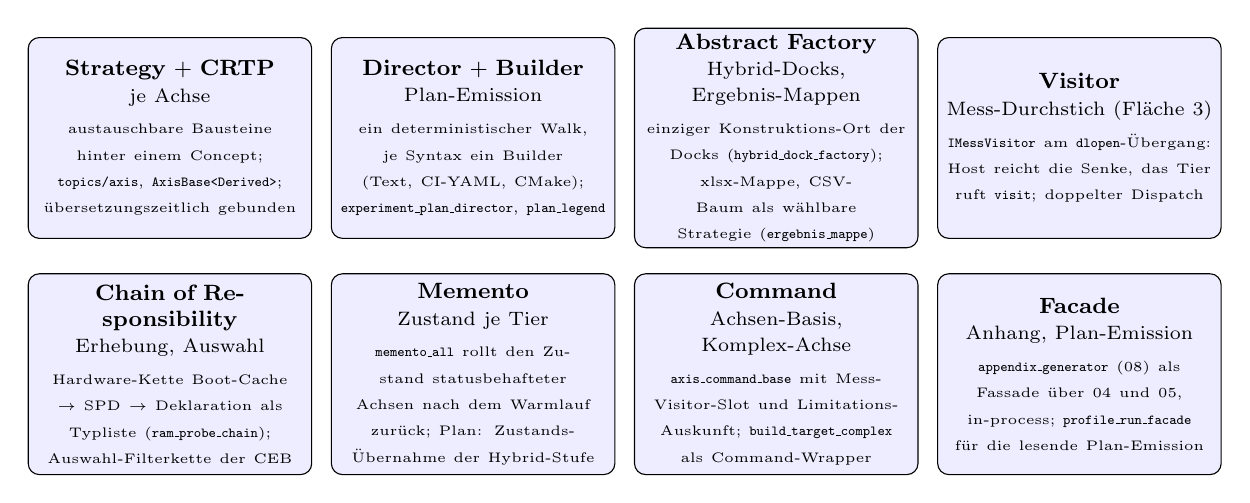
\begin{tikzpicture}[font=\footnotesize,
  mu/.style={draw,rounded corners,fill=blue!7,minimum width=3.6cm,minimum height=2.55cm,text width=3.4cm,align=center,inner sep=2pt}]
  \node[mu] (m1) at (0,0){\textbf{Strategy $+$ CRTP}\\{\scriptsize je Achse}\\[2pt]{\tiny austauschbare Bausteine hinter einem Concept; \texttt{topics/axis}, \texttt{AxisBase<Derived>}; übersetzungszeitlich gebunden}};
  \node[mu] (m2) at (3.85,0){\textbf{Director $+$ Builder}\\{\scriptsize Plan-Emission}\\[2pt]{\tiny ein deterministischer Walk, je Syntax ein Builder (Text, CI-YAML, CMake); \texttt{experiment\_plan\_director}, \texttt{plan\_legend}}};
  \node[mu] (m3) at (7.7,0){\textbf{Abstract Factory}\\{\scriptsize Hybrid-Docks, Ergebnis-Mappen}\\[2pt]{\tiny einziger Konstruktions-Ort der Docks (\texttt{hybrid\_dock\_factory}); xlsx-Mappe, CSV-Baum als wählbare Strategie (\texttt{ergebnis\_mappe})}};
  \node[mu] (m4) at (11.55,0){\textbf{Visitor}\\{\scriptsize Mess-Durchstich (Fläche 3)}\\[2pt]{\tiny \texttt{IMessVisitor} am \texttt{dlopen}-Übergang: Host reicht die Senke, das Tier ruft \texttt{visit}; doppelter Dispatch}};
  \node[mu] (m5) at (0,-3.0){\textbf{Chain of Responsibility}\\{\scriptsize Erhebung, Auswahl}\\[2pt]{\tiny Hardware-Kette Boot-Cache $\to$ SPD $\to$ Deklaration als Typliste (\texttt{ram\_probe\_chain}); Auswahl-Filterkette der CEB}};
  \node[mu] (m6) at (3.85,-3.0){\textbf{Memento}\\{\scriptsize Zustand je Tier}\\[2pt]{\tiny \texttt{memento\_all} rollt den Zustand statusbehafteter Achsen nach dem Warmlauf zurück; Plan: Zustands-Übernahme der Hybrid-Stufe}};
  \node[mu] (m7) at (7.7,-3.0){\textbf{Command}\\{\scriptsize Achsen-Basis, Komplex-Achse}\\[2pt]{\tiny \texttt{axis\_command\_base} mit Mess-Visitor-Slot und Limitations-Auskunft; \texttt{build\_target\_complex} als Command-Wrapper}};
  \node[mu] (m8) at (11.55,-3.0){\textbf{Facade}\\{\scriptsize Anhang, Plan-Emission}\\[2pt]{\tiny \texttt{appendix\_generator} (08) als Fassade über 04 und 05, in-process; \texttt{profile\_run\_facade} für die lesende Plan-Emission}};
\end{tikzpicture}
\caption[Das Register der Entwurfsmuster]{Das Register der Entwurfsmuster des Apparats (Benennung nach Gamma et al.): je Muster die Rolle
und der Code-Ort. Alle acht sind übersetzungszeitlich ausgeführt --- Bindung über Concepts, CRTP und
Typlisten statt über virtuelle Aufrufe ---, weil Tier-Binaries keine Laufzeit-Verzweigung zwischen
Bausteinen enthalten dürfen.}\label{fig:muster}
\end{figure}

%% INTERN-272: KA-085
Die Hybrid-Stufe ist die vierte Träger-Stufe (Abschnitt~\ref{sec:heuristics-modes}); ihr Code-Stand liegt
unter \texttt{hybrid/} (Abbildung~\ref{fig:hybrid-dock}). Implementiert sind die Dock-Verträge --- vier
Vertragsformen \texttt{standard}, \texttt{rollback}, \texttt{scan} und \texttt{resource\_control} als
\texttt{constexpr}-Registry mit sechzehn Status-Konstanten (\texttt{ok} und fünfzehn benannte
Ablehnungsgründe) ---, das minimale Prüf-Dock, die Dock-Factory als einziger Konstruktions-Ort, das
Dock-Array mit \texttt{HybridDockVariant} (die eine erlaubte variant-Stelle,
Abschnitt~\ref{sec:axes-impl}) und dem Laufzeit-Deckel \texttt{max\_docks}, der das $(N+1)$-te Andocken
mit \enquote{Array voll} abweist, der Parser der \texttt{<hybrid\_tier>}-Sektion (Zweiweg-Schalter
\texttt{enabled}, exklusiv je Kette, \texttt{max\_docks} Pflicht bei eingeschalteter Stufe) und der
Binary-Proxy, der eine Hybrid-.so nach außen zu einer gewöhnlichen Tier-Binary macht: Er erfüllt
\texttt{IAnatomyBase}, hält das Dock-Array und leitet den Antrieb an das Ziel durch, das an einem Dock
steckt. Nicht implementiert sind der \texttt{.so}-Export der Hybrid-Stufe (er hängt an einer offenen
Schichtungs-Auflage, weil eine Hybrid-.so Builder-Code linken müsste), die Eviction und der Router (er
braucht tatsächliche Messkurven). Gemessen an der Dateiliste, die die \texttt{README} des Verzeichnisses
\texttt{hybrid/} für die Dock-, Proxy- und Router-Schicht vorsieht, sind sechs der neun Dateien implementiert
(Dock-Verträge, Prüf-Dock, Dock-Factory, Dock-Array, XML-Parser, Binary-Proxy) und drei nicht (das Tier-Modul
des \texttt{.so}-Exports --- die zwei Modulquellen unter \texttt{tests/unit} belegen nur die Baubarkeit des
Modul-ABI ---, die Eviction und der Router); daneben führt das Verzeichnis die vier Header der
Klassifikations-Schicht (Klassifikation, Concept-Gate, Strategie je Genus, Synthese-Matrix) und drei weitere
Header für das Andocken, das Modul-ABI und die Stempel-Kette, insgesamt dreizehn Header.
Die Hybrid Module ABI v1 exportiert dieselben Pflicht-Symbole wie die plain
Tiere samt Gattung und Genus, und \texttt{comdare\_anatomy\_genus} meldet den \emph{Ziel}-Genus (das, was
das Modul für den Aufrufer ist), nie den Reroute-Genus der Klassifikation --- derselbe
gattungsunabhängige Loader lädt die Hybrid-.so über die eine Ladestrecke; die Stempel-Kette der
Hybrid-Stufe und die Hybrid-Positionen des Mess-Gate-Glieds (\texttt{hm}/\texttt{hmi}) führen ihre
Identität, und die Genus-Bau-Zulassung führt sechs Einträge, den sechsten für das Reroute-Genus mit dem
Dock-Deckel (Default 32) als Arität. Das Hybrid-Live-Ranking ist als vierte
Auswertungs-Komponente der compare-Stufe vorgesehen, und der Zustandsabgleich der Hybrid-Stufe ist per
Memento mit zwei Release-Artefakten, single und hybrid, im Lager vorgesehen
(Abschnitt~\ref{sec:heuristics-modes}); Umsetzungsstand: beides ist nicht implementiert, ebenso nicht die
Behebung der Schema-Drift, dass das XSD die \texttt{<hybrid\_tier>}-Sektion nicht führt. Der Hybrid-Modus kompiliert nur mithilfe der CEB\@.
\begin{figure}[htbp]\centering
%% INTERN-272: KA-086
\begin{tikzpicture}[font=\footnotesize,>=Stealth,
  hb/.style={draw,rounded corners,fill=blue!7,text width=2.9cm,minimum height=1.0cm,align=center,inner sep=2pt,font=\scriptsize},
  dk/.style={draw,rounded corners,fill=orange!12,text width=1.95cm,minimum height=1.1cm,align=center,inner sep=2pt,font=\tiny},
  ex/.style={draw,rounded corners,fill=green!8,text width=2.6cm,minimum height=1.0cm,align=center,inner sep=2pt,font=\tiny}]
  \node[draw,rounded corners,dashed,minimum width=9.0cm,minimum height=5.4cm] (frame) at (0,-0.4){};
  \node[font=\bfseries\scriptsize,anchor=north west] at (-4.5,2.3){Hybrid-\texttt{.so} (Gattung HeuristikAdapter, Reroute-Genus)};
  \node[hb] (proxy) at (-2.4,0.9){\texttt{HybridBinaryProxy}\\erfüllt \texttt{IAnatomyBase}; leitet den Antrieb an das Ziel-Dock durch};
  \node[hb] (arr) at (2.3,0.9){\texttt{DockArray\{\allowbreak max\_docks\}}\\\texttt{HybridDockVariant}: die eine erlaubte variant-Stelle};
  \draw[->,thick] (proxy)--(arr);
  \node[dk] (d1) at (-3.2,-1.4){Dock 1\\Vertrag \texttt{standard}\\$\to$ Ziel-Tier};
  \node[dk] (d2) at (-1.0,-1.4){Dock 2\\Vertrag \texttt{rollback}\\$\to$ Ziel-Tier};
  \node[dk] (d3) at (1.2,-1.4){Dock 3\\Vertrag \texttt{scan}\\$\to$ Ziel-Tier};
  \node[dk] (d4) at (3.4,-1.4){Dock $N$\\Vertrag \texttt{resource\_\allowbreak control}\\$\to$ Ziel-Tier};
  \draw[->] (arr)--(d1); \draw[->] (arr)--(d2); \draw[->] (arr)--(d3); \draw[->] (arr)--(d4);
  \node[font=\tiny,text=red!60!black] at (0.1,-2.55){Andocken $N+1$: Status \texttt{array\_voll} (Laufzeit-Deckel \texttt{max\_docks})};
  \node[ex] (fac) at (-6.3,0.9){\texttt{HybridDockFactory}\\Abstract Factory: einziger Konstruktions-Ort der Docks};
  \draw[->,dashed] (fac)--(proxy);
  \node[ex] (xml) at (-6.3,-1.4){\texttt{<hybrid\_tier enabled=true max\_docks=N>}\\Parser: \texttt{enabled} exklusiv je Kette, \texttt{max\_docks} Pflicht};
  \draw[->,dashed] (xml)--(d1);
  \node[ex] (sym) at (6.3,0.9){Exporte: sieben Pflicht-Symbole wie plain Tiere; \texttt{genus()} meldet den Ziel-Genus (Weg C)};
  \draw[->,dashed] (frame.east)--(sym);
  \node[ex] (st) at (6.3,-1.4){Stempel-Kette der Hybrid-Stufe; Mess-Gate-Felder \texttt{hm}/\texttt{hmi}; Genus-Bau-Zulassung: 6.\ Eintrag};
\end{tikzpicture}
\caption[Die Hybrid-Stufe im Code]{Die Hybrid-Stufe im Code: Der Binary-Proxy macht die Hybrid-.so nach außen zu einer
gewöhnlichen Tier-Binary und hält das Dock-Array mit dem Laufzeit-Deckel \texttt{max\_docks}; je Dock gilt
einer von vier Verträgen, die Dock-Factory ist der einzige Konstruktions-Ort, die
\texttt{<hybrid\_tier>}-Sektion der XML schaltet die Stufe und setzt den Deckel. Die Exporte sind
buchstabengleich zu den plain Tieren, \texttt{genus()} meldet den Ziel-Genus. Nicht implementiert: \texttt{.so}-Export,
Eviction, Router.}\label{fig:hybrid-dock}
\end{figure}

%% INTERN-272: KA-087
Das Lager (Abschnitt~\ref{sec:lager}) hat im Code ein übersetzungsstatisches Schlüssel-Schema
(\texttt{bestand\_\allowbreak{}schluessel\_\allowbreak{}schema}), das die vier Bestände deklariert, ohne
selbst Lager-Mechanik zu implementieren: Bestand~1, die Binaries, ist über eine Schlüssel-Politik geschlüsselt,
deren einziger SHA-512-Schlüssel mit dem Tier-Fingerprint identisch ist, die Zelle daneben geklammert;
Bestand~2, die Messwerte, über den 128-Hex-Fingerprint der vermessenen Binary und die Hardware-Identität
der messenden Maschine, die Zelle daneben geklammert und nie in den Digest fusioniert; Bestand~3, die
Synthese-Batches, und Bestand~4, die Lösungen, sind als Arbeitsschritt des Lager-Vollausbaus deklariert
(Tabelle~\ref{tab:lager-schluessel}). Drift zwischen Schema und Mechanik bricht beim Bau der Mechanik,
nicht erst im Lager. Der Versions-Lock (\texttt{axis\_version.lock}, Format v3, 719 Datensätze zu je drei
Zeilen) bindet jede Quell-Datei der Achsen --- die Heuristik-Header und den Overlay-Schnitt, über den das
Overlay-Glied des Tier-Fingerprints hasht --- an ihren Inhalts-Digest und ihre gestempelte
Algorithmus-Version: Eine Abweichung zwischen Lock und Discovery ist ein Fehlschlag, eine Rückstufung eines
versionstragenden Headers auf Digest-only ist ein Fehlschlag ohne Schreibweg, eine Aufwertung ist legitim und
verlangt die bewusste Neuerzeugung des Locks; das Gate \texttt{contract:axis-version-lock} der CI erzwingt das. Aus
dem Schema folgen die Lager-Eigenschaften des Konzepts: Die Messung ist immer eingeschaltet, im Lager wird
nur nachgemessen, was dort fehlt; ein Versionswechsel einer Achse ändert Stempel und Fingerprint und baut
den betroffenen Lager-Stapel neu; und weil die Hardware-Identität im Messwert-Schlüssel steht, hat jeder
Maschinentyp seinen eigenen Messwert-Bestand. Umsetzungsstand: Schema, Lock und die Bestände~1 und~2
sind implementiert; der Vollausbau --- Planer-Blattfunktion, CEB-Vollplatzierung, Hybrid-Ablage, Commit-Skip,
Neubau-Flag, XML-Zielwahl --- und die Binaries mit und ohne Messfühler samt Kurven-Dateien als
Lager-Einträge sind vorgesehen, aber nicht implementiert.
\begin{table}[htbp]\centering\footnotesize
\begin{tabular}{@{}lp{6.2cm}p{3.0cm}p{2.6cm}@{}}
\toprule
Bestand & Schlüssel-Komponenten & Quelle im Code & Umsetzungsstand \\
\midrule
1 Binaries & der eine SHA-512-Schlüssel ($=$ Tier-Fingerprint); Zell-Klammer daneben & Schlüssel-Politik des Bestandslogs & implementiert \\
2 Messwerte & 128-Hex-Fingerprint der vermessenen Binary; Hardware-Identität der messenden Maschine; Zelle daneben geklammert, nie fusioniert & Messwert-Schlüsselquelle des Bestandslogs & implementiert \\
3 Synthese-Batches & Maschine; Voll-Stempel; Referenz auf Mess-Ebene und Kanal & Schema deklariert & nicht implementiert (Vollausbau) \\
4 Lösungen & kanonisierter Hash der Anwender-XML\@; Maschine; Referenzen auf die beteiligten Bestände & Schema deklariert & nicht implementiert (Vollausbau) \\
\bottomrule
\end{tabular}
\caption{Die vier Lager-Bestände und ihre Schlüssel-Komponenten nach dem übersetzungsstatischen
Schlüssel-Schema; der Versions-Lock bindet die Achsen-Quellen an Digest und gestempelte
Version.}\label{tab:lager-schluessel}
\end{table}

Damit ist der Apparat vollständig beschrieben --- von den vier Repositorien über den Prüfling, die
achtzehn Organ-Achsen und die Träger-Stufenkette bis zur Kette vom Plan zur Tier-Binary, ihren
Vertrags-Flächen, der schichtweisen Qualitätssicherung, den Realm-Wurzeln im Code, dem Muster-Register,
der Hybrid-Stufe und dem Lager. Kapitel~\ref{ch:eval} legt die Methodik offen, mit der dieser Apparat
bewertet wird.
